% Options for packages loaded elsewhere
\PassOptionsToPackage{unicode}{hyperref}
\PassOptionsToPackage{hyphens}{url}
%
\documentclass[
]{article}
\usepackage{amsmath,amssymb}
\usepackage{iftex}
\ifPDFTeX
  \usepackage[T1]{fontenc}
  \usepackage[utf8]{inputenc}
  \usepackage{textcomp} % provide euro and other symbols
\else % if luatex or xetex
  \usepackage{unicode-math} % this also loads fontspec
  \defaultfontfeatures{Scale=MatchLowercase}
  \defaultfontfeatures[\rmfamily]{Ligatures=TeX,Scale=1}
\fi
\usepackage{lmodern}
\ifPDFTeX\else
  % xetex/luatex font selection
\fi
% Use upquote if available, for straight quotes in verbatim environments
\IfFileExists{upquote.sty}{\usepackage{upquote}}{}
\IfFileExists{microtype.sty}{% use microtype if available
  \usepackage[]{microtype}
  \UseMicrotypeSet[protrusion]{basicmath} % disable protrusion for tt fonts
}{}
\makeatletter
\@ifundefined{KOMAClassName}{% if non-KOMA class
  \IfFileExists{parskip.sty}{%
    \usepackage{parskip}
  }{% else
    \setlength{\parindent}{0pt}
    \setlength{\parskip}{6pt plus 2pt minus 1pt}}
}{% if KOMA class
  \KOMAoptions{parskip=half}}
\makeatother
\usepackage{xcolor}
\usepackage[left=1.5in, right=1.5in, top=1in, bottom=1in]{geometry}
\usepackage{longtable,booktabs,array}
\usepackage{calc} % for calculating minipage widths
% Correct order of tables after \paragraph or \subparagraph
\usepackage{etoolbox}
\makeatletter
\patchcmd\longtable{\par}{\if@noskipsec\mbox{}\fi\par}{}{}
\makeatother
% Allow footnotes in longtable head/foot
\IfFileExists{footnotehyper.sty}{\usepackage{footnotehyper}}{\usepackage{footnote}}
\makesavenoteenv{longtable}
\usepackage{graphicx}
\makeatletter
\newsavebox\pandoc@box
\newcommand*\pandocbounded[1]{% scales image to fit in text height/width
  \sbox\pandoc@box{#1}%
  \Gscale@div\@tempa{\textheight}{\dimexpr\ht\pandoc@box+\dp\pandoc@box\relax}%
  \Gscale@div\@tempb{\linewidth}{\wd\pandoc@box}%
  \ifdim\@tempb\p@<\@tempa\p@\let\@tempa\@tempb\fi% select the smaller of both
  \ifdim\@tempa\p@<\p@\scalebox{\@tempa}{\usebox\pandoc@box}%
  \else\usebox{\pandoc@box}%
  \fi%
}
% Set default figure placement to htbp
\def\fps@figure{htbp}
\makeatother
\setlength{\emergencystretch}{3em} % prevent overfull lines
\providecommand{\tightlist}{%
  \setlength{\itemsep}{0pt}\setlength{\parskip}{0pt}}
\setcounter{secnumdepth}{5}
\usepackage{booktabs}
\usepackage{threeparttable}
\usepackage[utf8]{inputenc}
\usepackage[T1]{fontenc}
\usepackage{amsmath}
\usepackage{tabularx}
\usepackage{threeparttable}
\usepackage{pdflscape}
\usepackage{float}
\floatplacement{figure}{H}
\usepackage{subcaption}
\usepackage{caption}
\captionsetup[figure]{skip=0.5em}
\usepackage{booktabs}
\usepackage{longtable}
\usepackage{array}
\usepackage{multirow}
\usepackage{wrapfig}
\usepackage{float}
\usepackage{colortbl}
\usepackage{pdflscape}
\usepackage{tabu}
\usepackage{threeparttable}
\usepackage{threeparttablex}
\usepackage[normalem]{ulem}
\usepackage{makecell}
\usepackage{xcolor}
\usepackage[]{natbib}
\bibliographystyle{apalike}
\usepackage{bookmark}
\IfFileExists{xurl.sty}{\usepackage{xurl}}{} % add URL line breaks if available
\urlstyle{same}
\hypersetup{
  pdftitle={Imagine -- An Exploratory Analysis v2},
  hidelinks,
  pdfcreator={LaTeX via pandoc}}

\title{Imagine -- An Exploratory Analysis v2}
\author{}
\date{\vspace{-2.5em}}

\begin{document}
\maketitle

\section{Data Merging, Filtering, and Data
Transformation}\label{data-merging-filtering-and-data-transformation}

Sense and feature annotation datasets were merged using \texttt{\$id}
and \texttt{\$no}, as suggested by Nina. Sense annotations by ARB were
ignored, since they only span 100 rows. Rows with non-numeric values in
either feature variable, non-NA value in \texttt{\$Exclusions} (from the
sense annotation data), or non-converging sense-annotations by NCH \& AH
were removed, leaving 868 observations. Further, rows with sense values
\texttt{"?-UNCLASSIFIABLE"}, \texttt{"5-EXCLAMATIVE"}, or
\texttt{"O-Other"} (not occurring) were dropped due to low occurrence
(see Table \ref{tab:senseCounts}), which makes estimation unstable. The
final dataset consists of 856 observations. Lastly, the three feature
dimensions were \(z\)-scaled for comparability.

\begin{table}[H]
\centering
\caption{\label{tab:unnamed-chunk-3}\label{tab:senseCounts} Sense counts before removal of edge classes.}
\centering
\begin{tabular}[t]{lr}
\toprule
Sense & N\\
\midrule
?-UNCLASSIFIABLE & 5\\
1-VIZUALIZE/PICTURE & 499\\
2-THINK/BELIVE & 211\\
3-SUPPOSE/ASSUME & 88\\
4-FALSE\_PERCEPTION & 58\\
5-EXCLAMATIVE & 7\\
\bottomrule
\end{tabular}
\end{table}

\section{Descriptive Statistics}\label{descriptive-statistics}

Figure \ref{fig:distributions} shows considerable overlap in feature
distributions across the different senses. To quantify this, we computed
pairwise overlap coefficients between sense distributions for each
feature using kernel density estimation (KDE), measuring both the raw
shared area under the minimum of two KDE curves and its normalization by
each sense's total density (see Table \ref{tab:overlap} in the
Appendix). Figure \ref{fig:Xdistributions} shows a similar picture for
feature interactions. In view of that, clear sense separation via
feature dimensions seems unlikely.

\begin{figure}[h]

{\centering 
\includegraphics[width=1\linewidth]{imagine_report_v2_files/figure-latex/unnamed-chunk-4-1} 

}

\caption{Fetaure distributions for the different senses\label{fig:distributions}}\label{fig:unnamed-chunk-4}
\end{figure}

\begin{figure}[h]

{\centering 
\includegraphics[width=1\linewidth]{imagine_report_v2_files/figure-latex/unnamed-chunk-5-1} 

}

\caption{Interactions of feature distributions for the different senses\label{fig:Xdistributions}}\label{fig:unnamed-chunk-5}
\end{figure}

\section{Predictive Modeling of Sense
Membership}\label{predictive-modeling-of-sense-membership}

To characterize how annotation dimensions jointly predict latent sense
membership, we fit a multinomial generalized linear model with ridge
(L2) regularization. Manual sense annotations served as the dependent
variable. Predictors included all three annotation dimensions and their
pairwise interactions. Regularization strength was selected via
cross-validation to promote coefficient stability.

The multinomial model achieved a cross-validated accuracy of 75.4\% with
optimal \(\lambda\)=0.033. Performance was highly uneven across senses,
however. Table \ref{tab:senseAccuracy} details accuracy per sense:

\begin{itemize}
\tightlist
\item
  \texttt{"1-VISUALIZE/PICTURE"} was recovered with high accuracy
  (97.4\%) and high posterior concentration
  (\(\tilde{p}_{\max}\)=0.825), indicating a well-defined feature
  region.
\item
  \texttt{"2-THINK/BELIEVE"} showed moderate accuracy (72.5\%) with
  correspondingly moderate confidence (\(\tilde{p}_{\max}\)=0.624).
\item
  \texttt{"3-SUPPOSE/ASSUME"} \& \texttt{"4-FALSE\_PERCEPTION"} were not
  reliably recovered (accuracy=0\% and 10.3\% respectively). Both were
  misclassified \texttt{"1-VISUALIZE/PICTURE"} or
  \texttt{"2-THINK/BELIEVE"} with low to moderate confidence
  (\(\tilde{p}_{\max}\)=0.652 and \(\tilde{p}_{\max}\)=0.577
  respectively).
\end{itemize}

\begin{table}[H]
\centering
\caption{\label{tab:unnamed-chunk-7}Posterior probability concentration and classification accuracy by sense. $\tilde{p}_{\max}$ denotes the median maximum predicted probability across observations; $\text{IQR}(\hat{p}_{\max})$ denotes the interquartile range of maximum predicted probabilities.\label{tab:senseAccuracy}}
\centering
\begin{tabular}[t]{lrrr}
\toprule
True Sense & $\tilde{p}_{\max}$ & $\text{IQR}(\hat{p}_{\max})$ & Accuracy\\
\midrule
1-VIZUALIZE/PICTURE & 0.825 & 0.187 & 0.974\\
2-THINK/BELIVE & 0.624 & 0.192 & 0.725\\
3-SUPPOSE/ASSUME & 0.652 & 0.154 & 0.000\\
4-FALSE\_PERCEPTION & 0.577 & 0.234 & 0.103\\
\bottomrule
\end{tabular}
\end{table}

Precision, recall, and F1 are reported in Table \ref{tab:cmDetail}. Note
that the precision and F1 for \texttt{"3-SUPPOSE/ASSUME"} is NA because
it was never correctly classified. Table \ref{tab:cm} in the Appendix
details the the confusion matrix by sense.

\begin{table}[H]
\centering
\caption{\label{tab:unnamed-chunk-8}Confusion Matrix.\label{tab:cmDetail}}
\centering
\begin{tabular}[t]{lrrr}
\toprule
  & Precision & Recall & F1\\
\midrule
Class: 1-VIZUALIZE/PICTURE & 0.7928222 & 0.9739479 & 0.8741007\\
Class: 2-THINK/BELIVE & 0.6566524 & 0.7251185 & 0.6891892\\
Class: 3-SUPPOSE/ASSUME &  & 0.0000000 & \\
Class: 4-FALSE\_PERCEPTION & 0.6000000 & 0.1034483 & 0.1764706\\
\bottomrule
\end{tabular}
\end{table}

These results indicate that the three features define a robust two-way
opposition between \texttt{"1-VISUALIZE/PICTURE"} and
\texttt{"2-THINK/BELIEVE"}, but are insufficient to distinguish the
remaining senses.

As a robustness check, we assessed coefficient stability using
nonparametric bootstrapping (500 resamples). Bootstrap confidence
intervals were narrow across main effects and interactions (Figure
\ref{fig:bootstrapping}), indicating that the fitted probability
surfaces were numerically stable under resampling. Keep in mind that
estimates for \texttt{"3-SUPPOSE/ASSUME"} and
\texttt{"FALSE\_PERCEPTION"} should be interpreted cautiously.

\begin{figure}[h]

{\centering 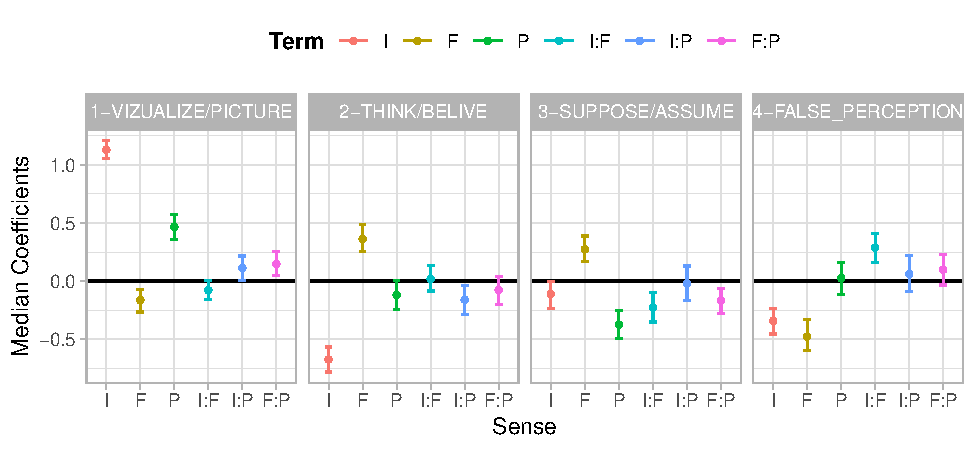
\includegraphics[width=1\linewidth]{imagine_report_v2_files/figure-latex/unnamed-chunk-9-1} 

}

\caption{Bootstrapped Coefficients (n = 500) with 95\% CI.\label{fig:bootstrapping}}\label{fig:unnamed-chunk-9}
\end{figure}

Predicted probabilities based on the optimal model were generated across
the observed range of each pair of annotation dimensions while holding
the third dimension constant at its median. These predictions were
visualized in Figure \ref{fig:Xeffects} as two-dimensional heatmaps to
facilitate interpretation of interaction patterns.

\begin{figure}[h]

{\centering 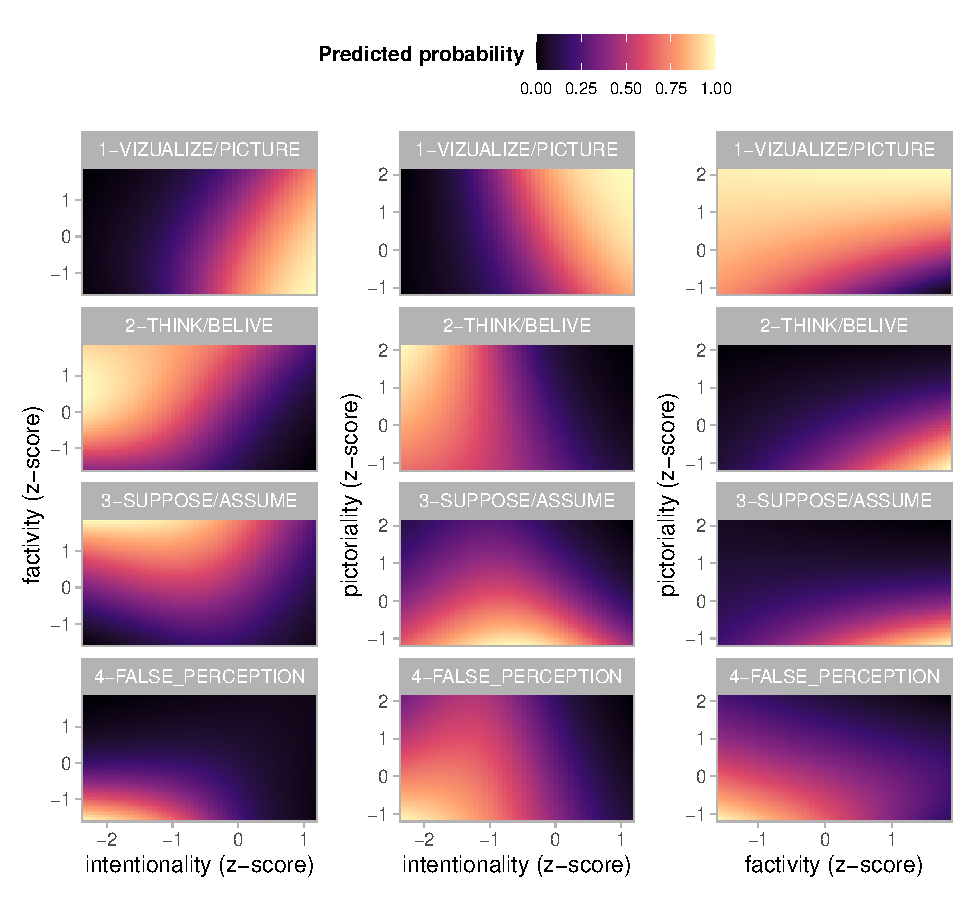
\includegraphics[width=1\linewidth]{imagine_report_v2_files/figure-latex/unnamed-chunk-10-1} 

}

\caption{redicted sense probability based on GLM with ridge regularization for 2-way interactions. The third dimension is held constant at the median value.\label{fig:Xeffects}}\label{fig:unnamed-chunk-10}
\end{figure}

\section{Embedding analysis}\label{embedding-analysis}

In addition to the statistical analysis, we leveraged contextual
embeddings of sentences containing the term \textit{imagine} to
investigate how different senses of the word are represented in latent
semantic space. This embedding analysis explores the geometric structure
of the representations, the relationship between semantic similarity and
sense membership, and the alignment of embeddings with the annotated
semantic dimensions. The approach provides a comprehensive view of how
contextual usage patterns are captured by the language model (BERT) and
how they relate to theoretical distinctions between senses.

\subsection{Sense overlap based on centroid
distance}\label{sense-overlap-based-on-centroid-distance}

For each sense, we computed the cosine distance of every
\textit{imagine} token embedding to its own sense centroid and to the
other sense centroids. We then estimated the kernel density (KDE)
distributions of these distances and calculated the overlap between the
densities. The resulting overlap scores quantify how well each sense
cluster is discriminated from the others in centroid space. Importantly,
this metric measures discriminability from cluster centers, not the
actual geometric overlap of the clusters themselves. It essentially
answers the question: ``If I pick a token at random from Sense 1, how
often could it be mistaken for Sense 2 based on centroid proximity?''
This approach does not account for the internal distribution of
embeddings within a cluster. Two clusters could substantially overlap in
the embedding space, yet the distance-to-centroid measure might still
suggest low overlap if tokens happen to be near their respective
centroids.

Figure \ref{fig:KDEdistanceCentroid_ownVSother} shows the cosine
distance of tokens for each sense to their own sense-centroid and the
other sense-centroids. The overlap fractions are detailed in Table
\ref{tab:coverlapfrac}.

\begin{figure}
    \centering
    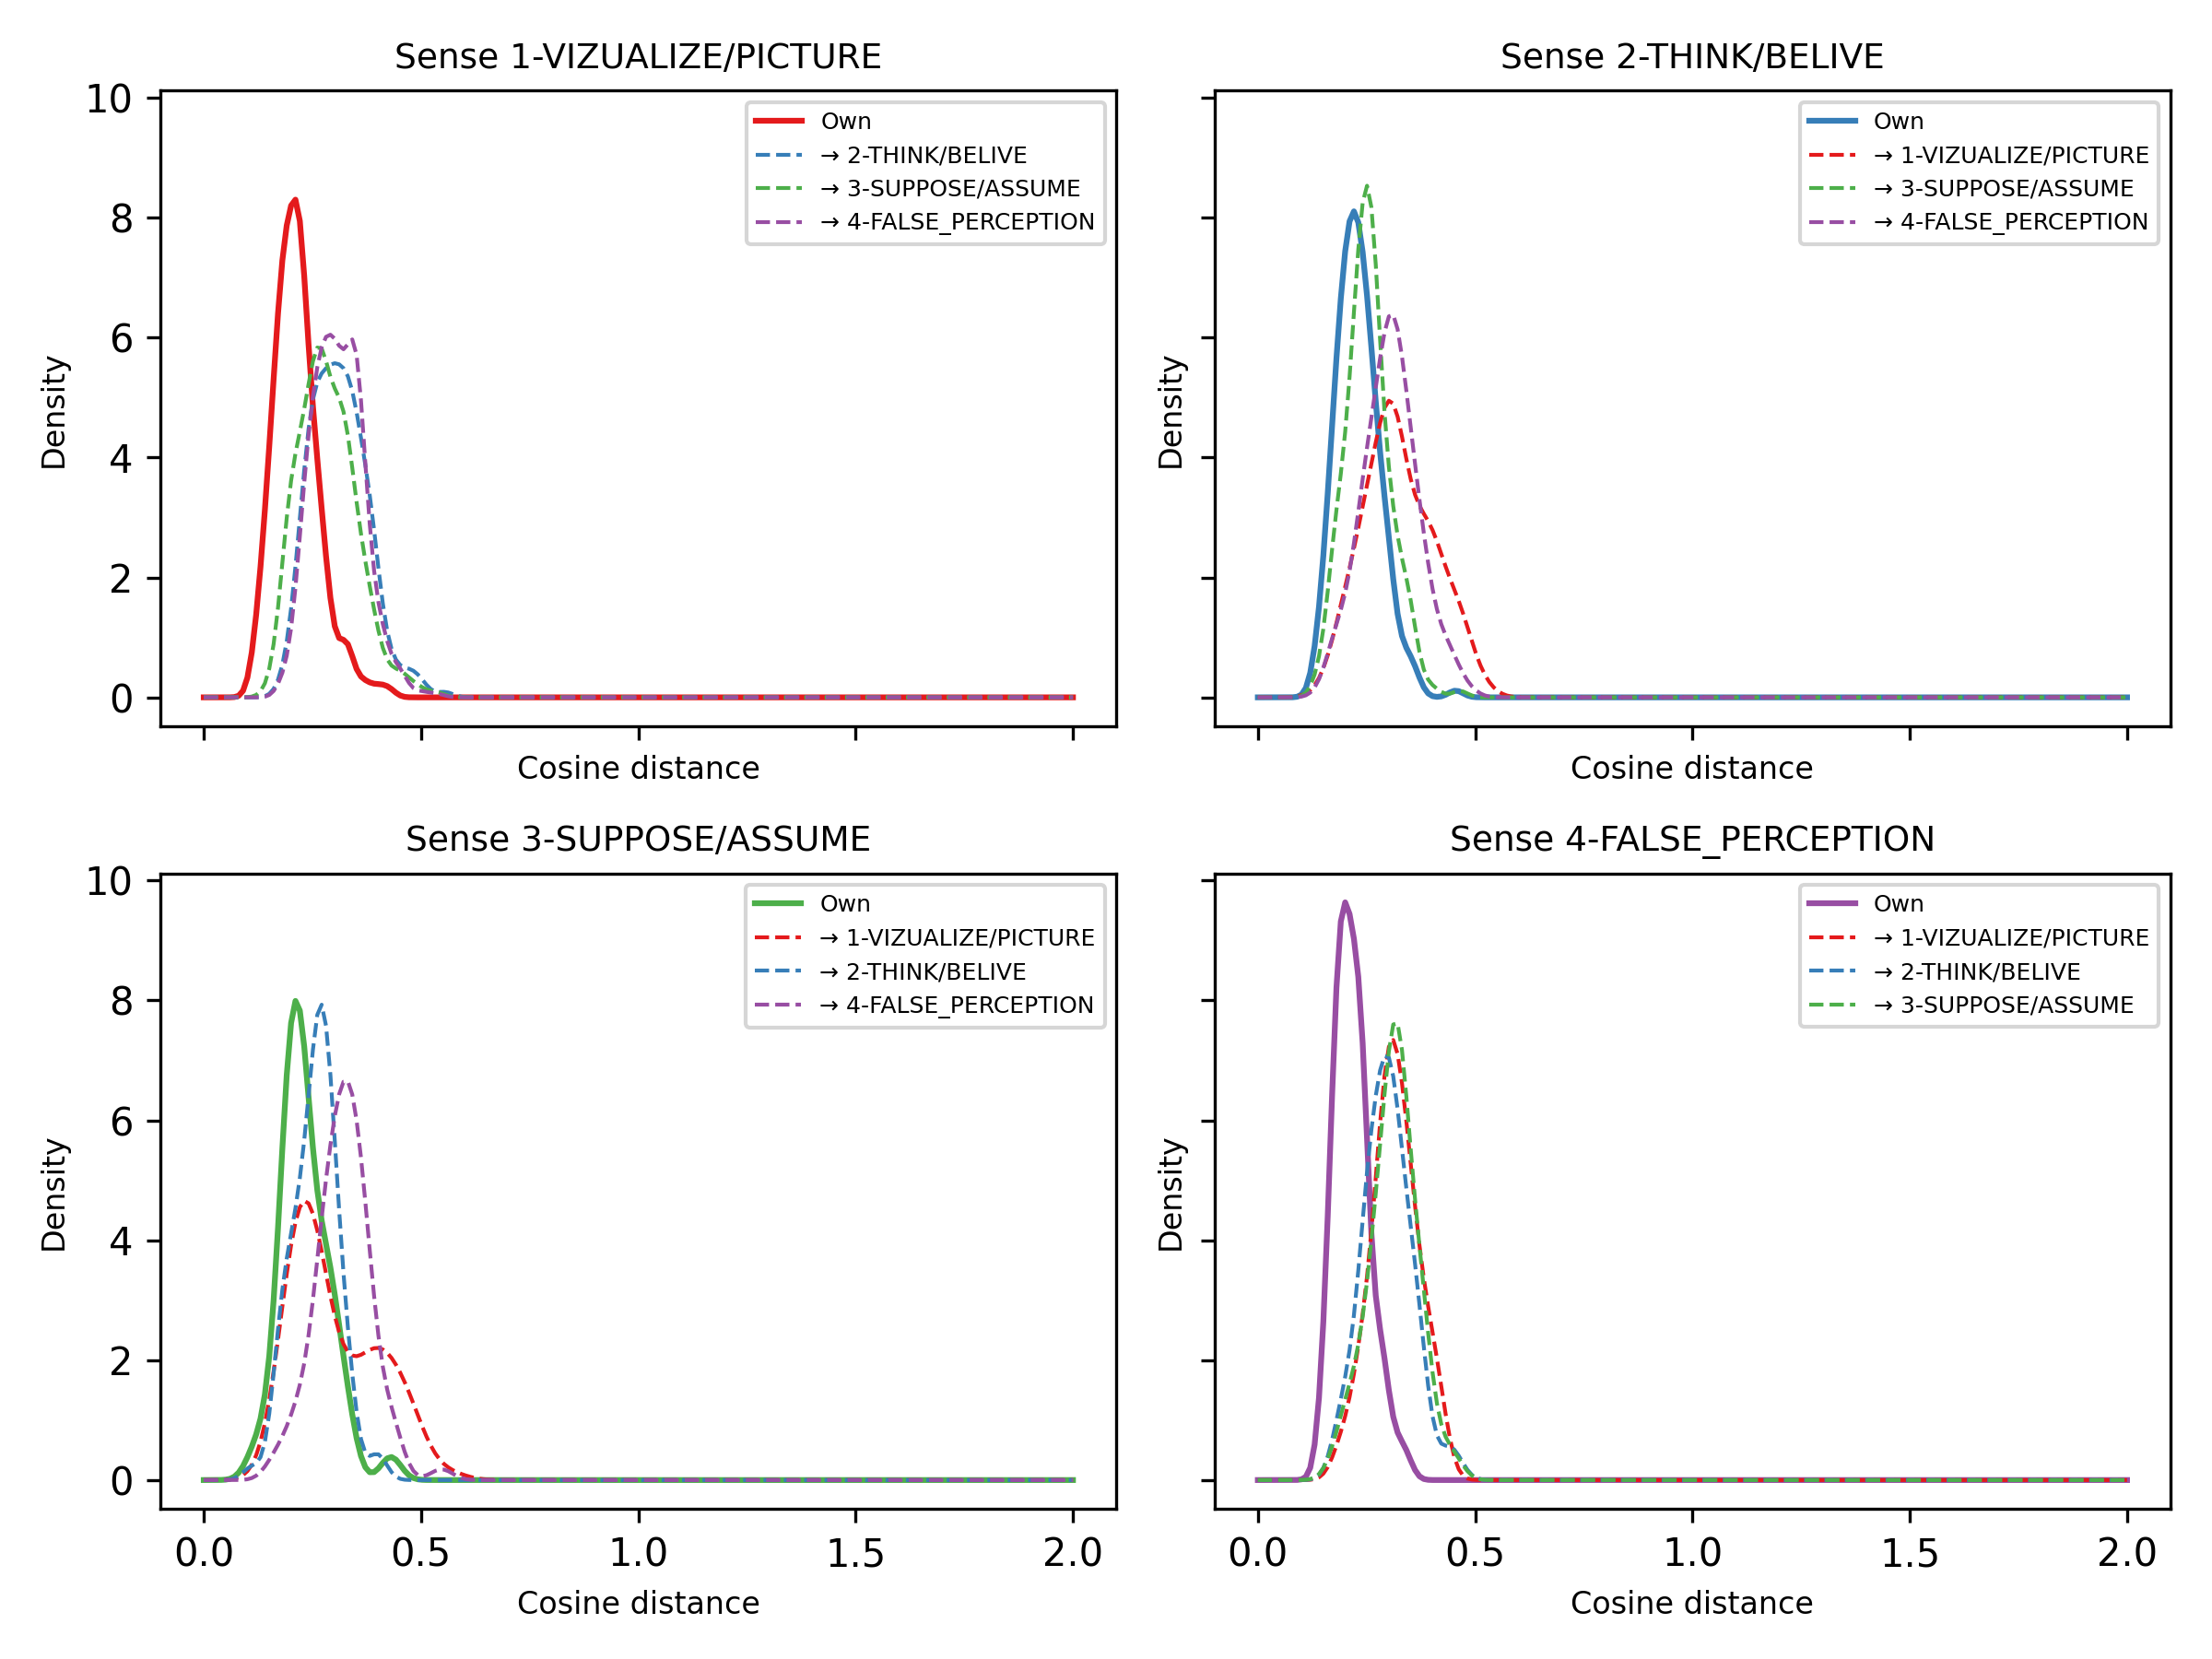
\includegraphics[width=0.8\linewidth]{../../output/plots/overlap_density_v2.png}
    \caption{Centroid-based overlap.}
    \label{fig:KDEdistanceCentroid_ownVSother}
\end{figure}

\begin{table}[H]
\centering
\caption{\label{tab:unnamed-chunk-11}1D KDE overlap fractions based on cosine distance to sense centroids.\label{tab:coverlapfrac}}
\centering
\begin{tabular}[t]{lllr}
\toprule
Sense 1 &  & Sense 2 & \%\\
\midrule
1-VIZUALIZE/PICTURE & vs & 2-THINK/BELIVE & 0.403\\
1-VIZUALIZE/PICTURE & vs & 3-SUPPOSE/ASSUME & 0.541\\
1-VIZUALIZE/PICTURE & vs & 4-FALSE\_PERCEPTION & 0.385\\
2-THINK/BELIVE & vs & 1-VIZUALIZE/PICTURE & 0.477\\
2-THINK/BELIVE & vs & 3-SUPPOSE/ASSUME & 0.801\\
2-THINK/BELIVE & vs & 4-FALSE\_PERCEPTION & 0.502\\
3-SUPPOSE/ASSUME & vs & 1-VIZUALIZE/PICTURE & 0.693\\
3-SUPPOSE/ASSUME & vs & 2-THINK/BELIVE & 0.755\\
3-SUPPOSE/ASSUME & vs & 4-FALSE\_PERCEPTION & 0.447\\
4-FALSE\_PERCEPTION & vs & 1-VIZUALIZE/PICTURE & 0.317\\
4-FALSE\_PERCEPTION & vs & 2-THINK/BELIVE & 0.404\\
4-FALSE\_PERCEPTION & vs & 3-SUPPOSE/ASSUME & 0.332\\
\bottomrule
\end{tabular}
\end{table}

\subsection{Geometric overlap}\label{geometric-overlap}

To complement the centroid-based distances, we also computed overlap
directly on the embedding distributions for each sense. For this, we
estimated KDE functions over the embeddings themselves (after 1D and 2D
PCA reduction). This yields how much of the geometric ``surface'' of one
cluster is occupied by the other. Unlike the centroid-based overlap,
which measures discriminability relative to cluster centers, this method
captures actual geometric overlap in embedding space. High overlap here
indicates that embeddings of the two senses physically occupy the same
regions, reflecting semantic entanglement or ambiguity. Low overlap
indicates that the clusters are well-separated in latent space,
regardless of centroid proximity. Thus, this analysis provides a more
direct estimate of semantic distinctiveness at the token level, whereas
centroid distances summarize separability from the average cluster
location. The overlap in 1D and 2D space is shown in Figure
\ref{fig:KDEsurface}. Table \ref{tab:kde1dfrac} \& \ref{tab:kde2dfrac}
detail the overlap fractions, for 1D and 2D respectively.

\begin{figure}
\centering
    \caption{Geometric overlap of different senses in embedding space.}
    \label{fig:KDEsurface}
    \begin{subfigure}[b]{0.6\textwidth}
    \centering
    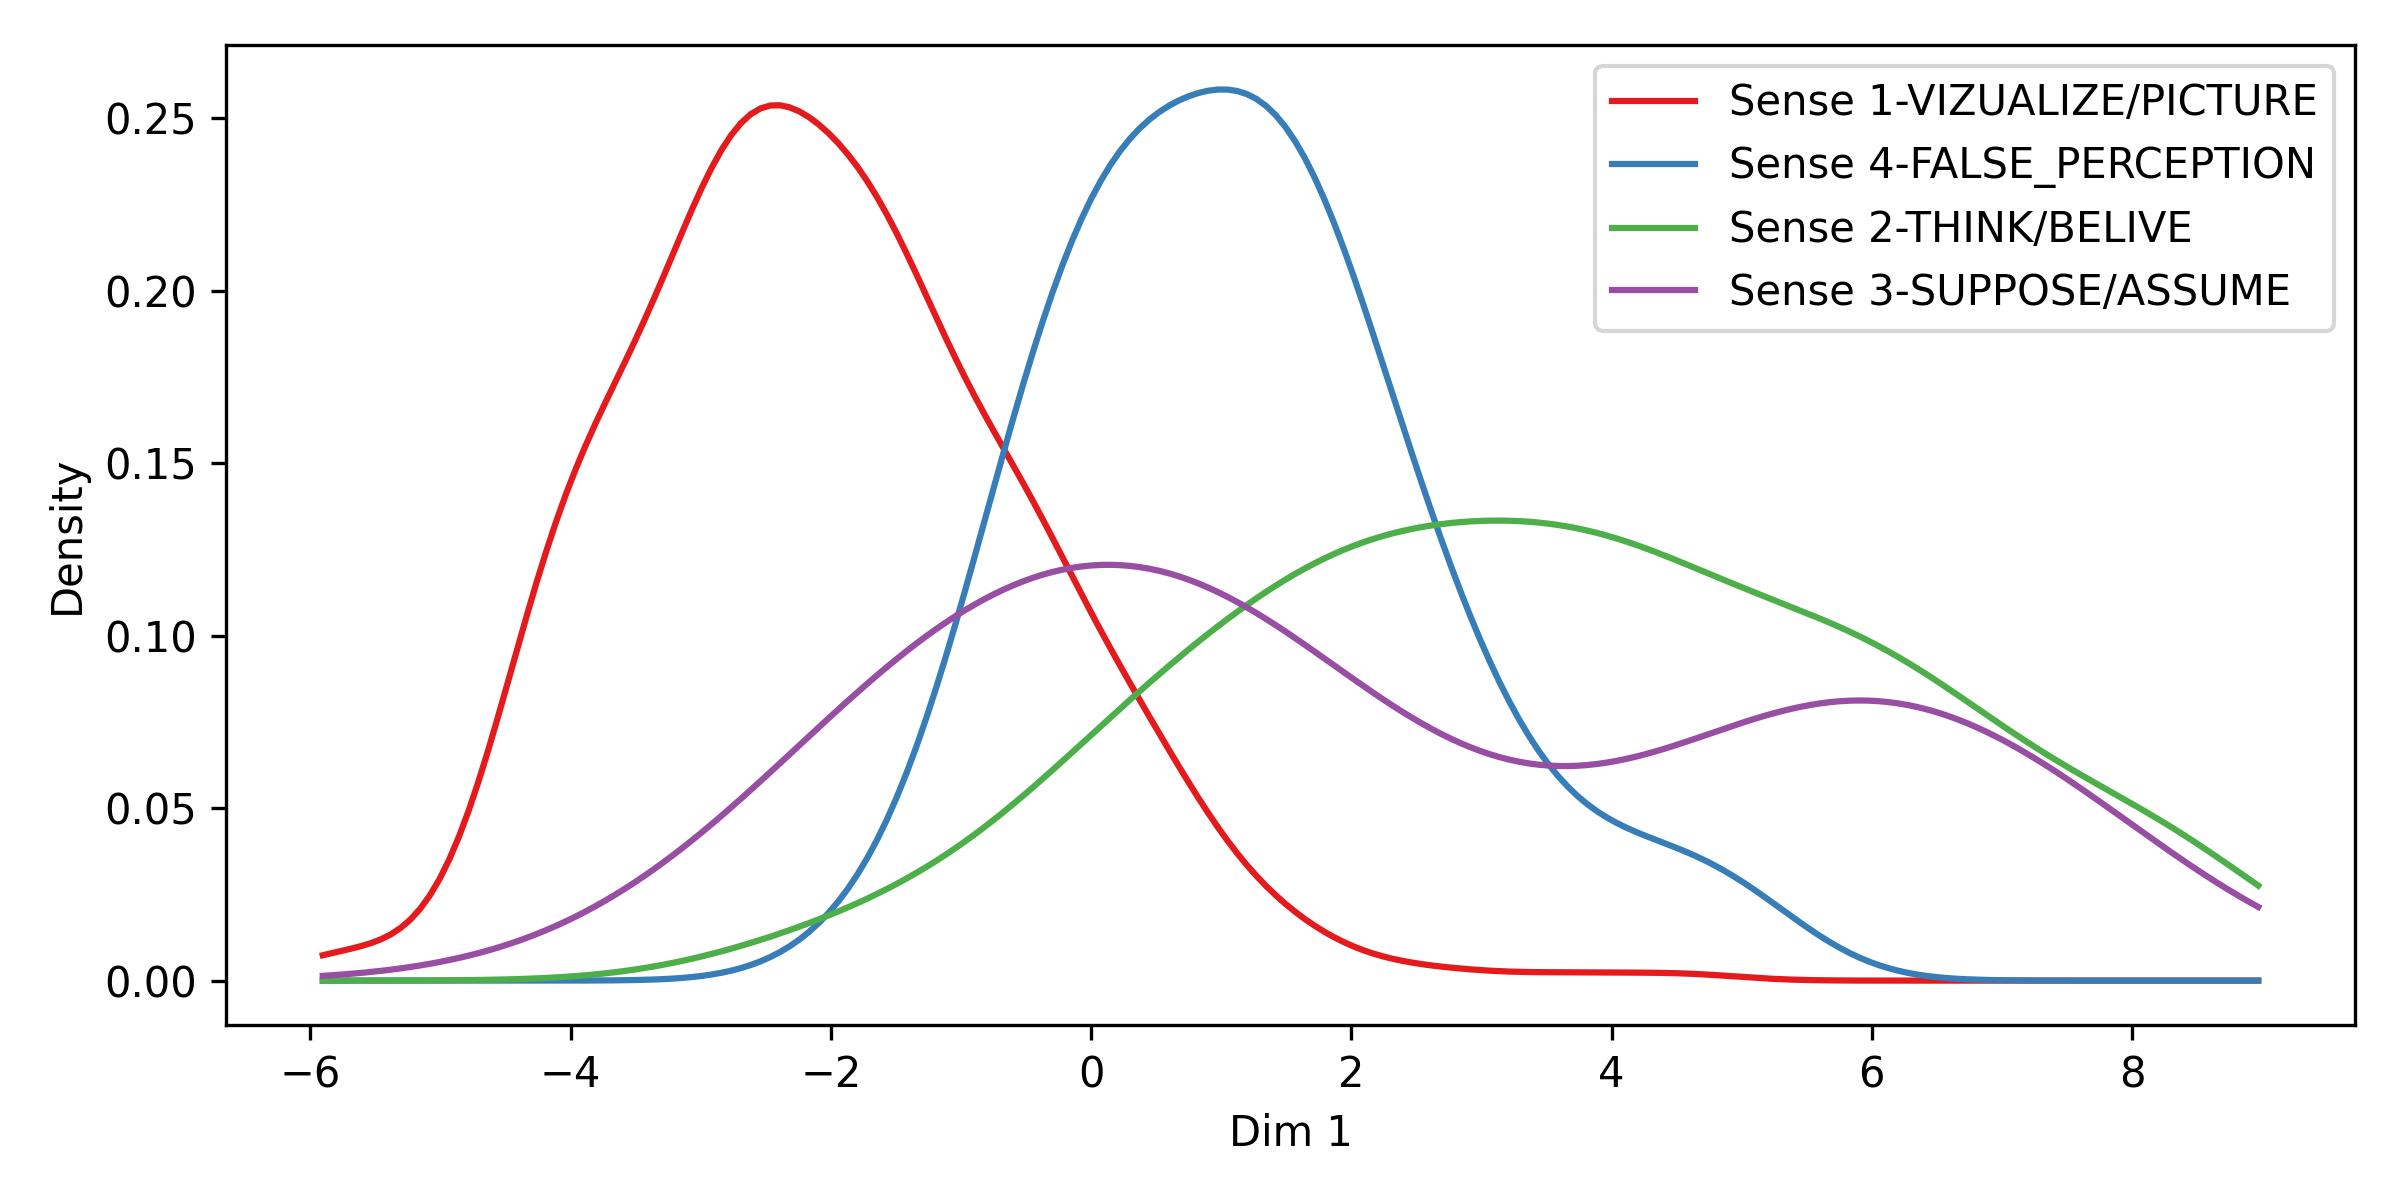
\includegraphics[width=\textwidth]{../../output/plots/kde1D_embeddings_overlap_v2.png}
    \caption{\label{fig:KDEsurface1D}}
    \end{subfigure}
    \hfill
    \begin{subfigure}[b]{0.38\textwidth}
    \centering
    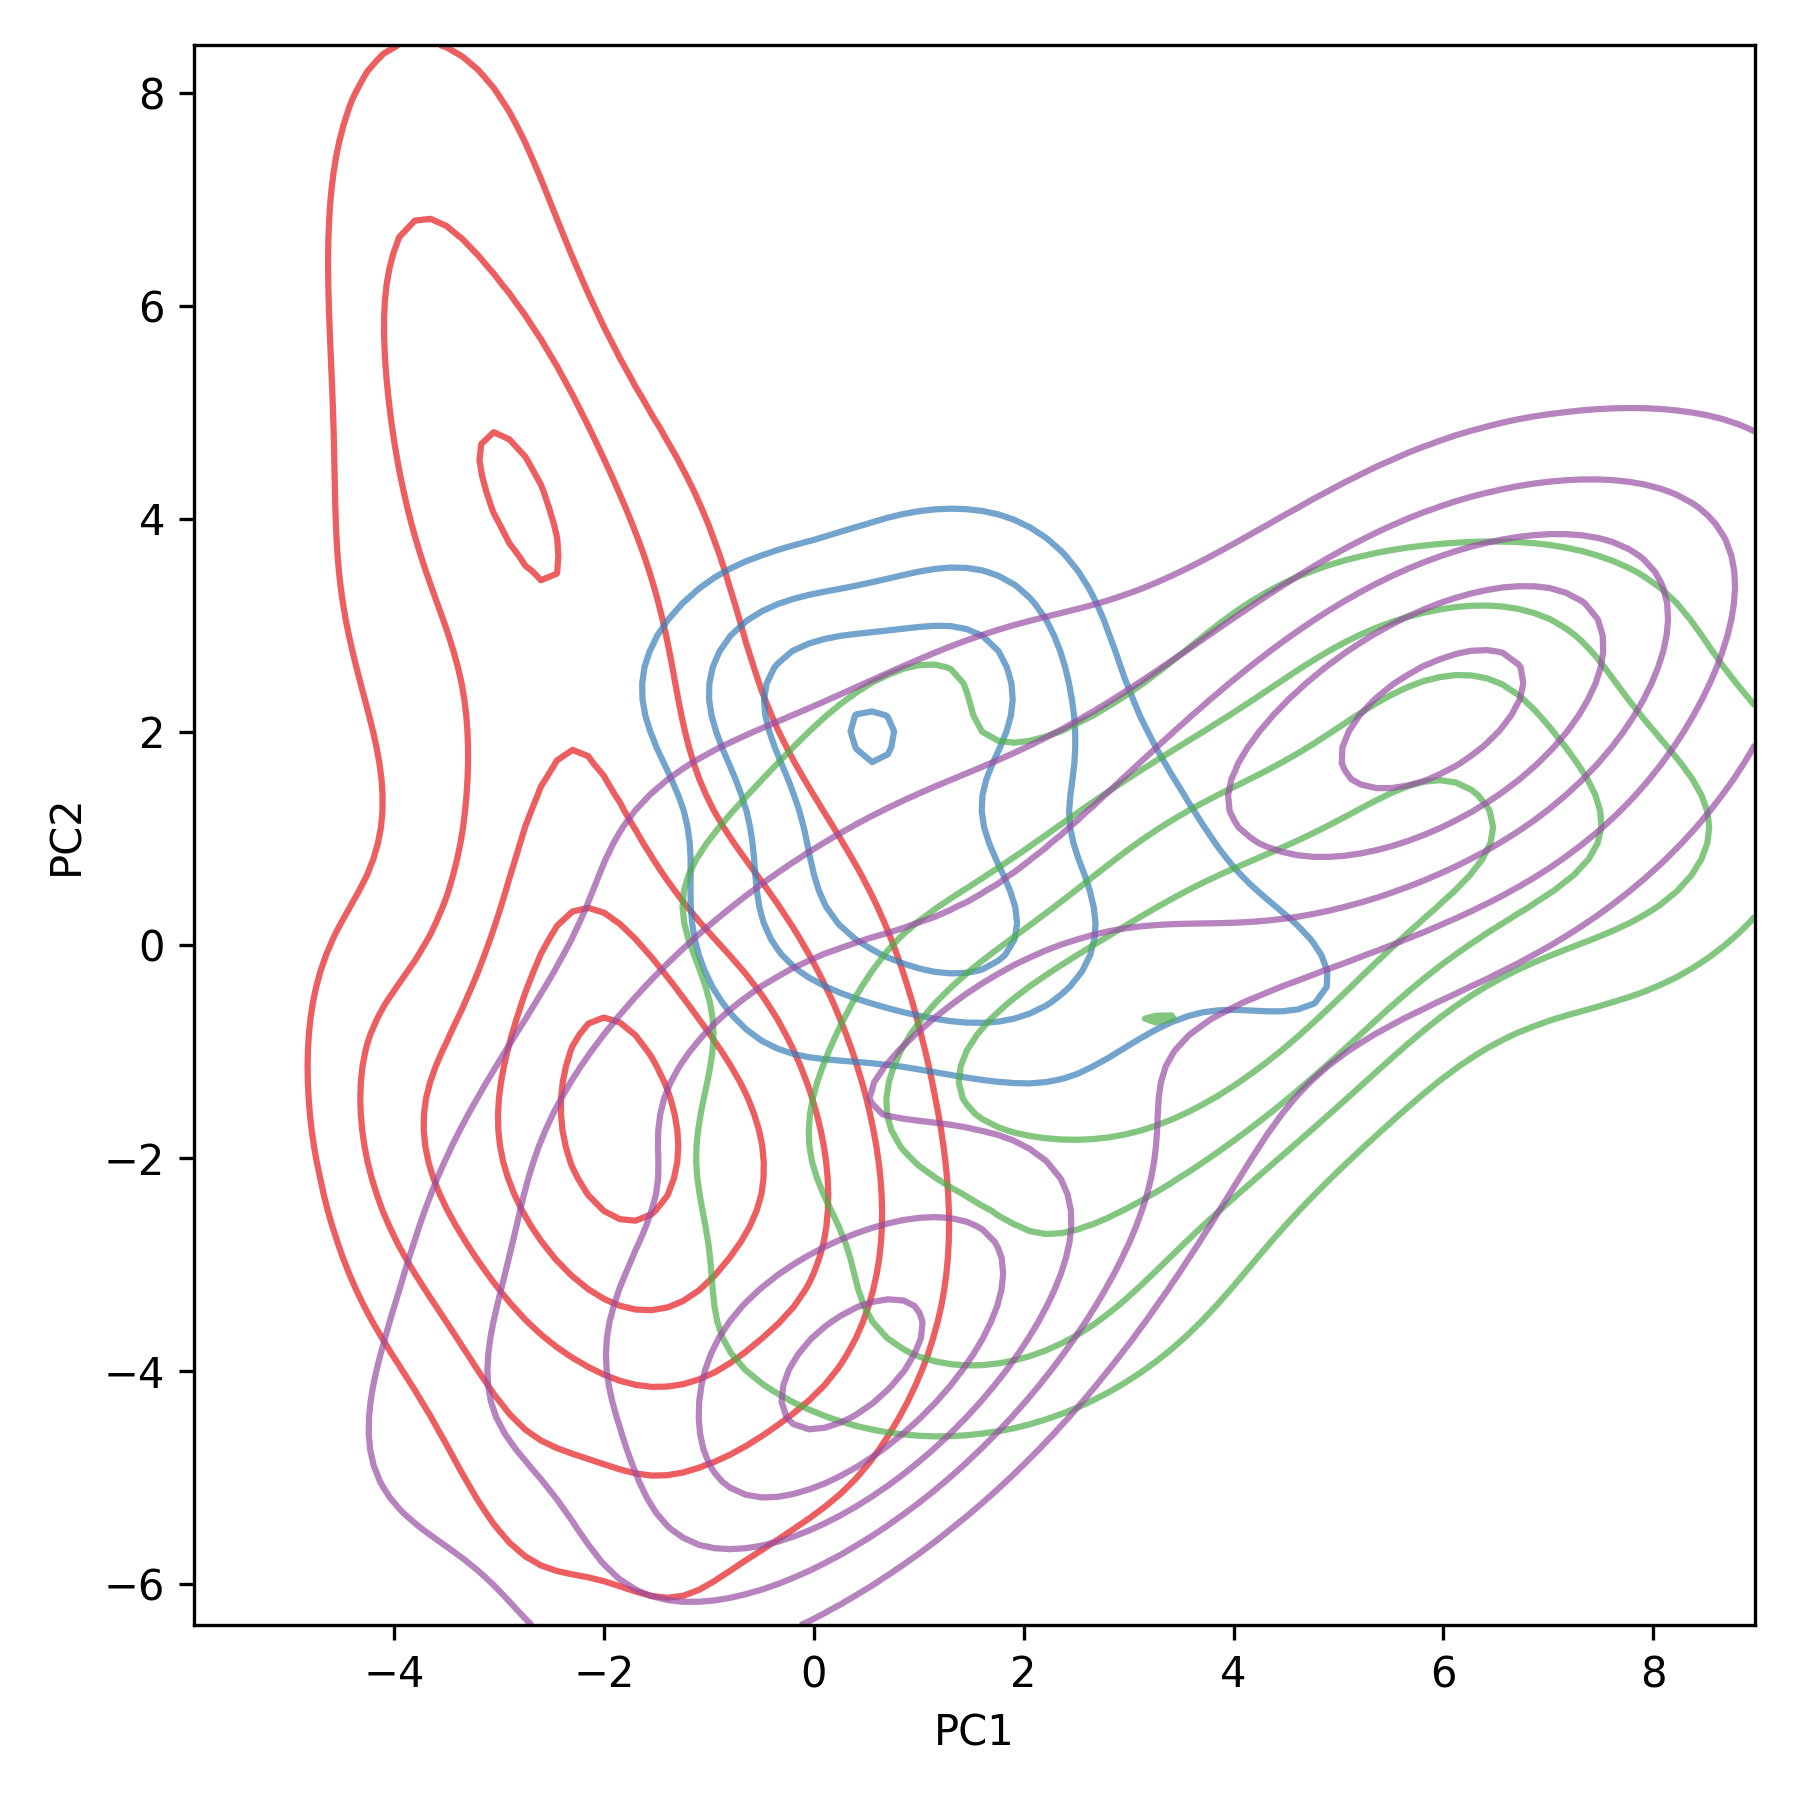
\includegraphics[width=0.9\textwidth]{../../output/plots/kde2D_embeddings_overlap_v2.png}
    \caption{\label{fig:KDEsurface1D}}
    \end{subfigure}
\end{figure}

\begin{table}[H]
\centering
\caption{\label{tab:unnamed-chunk-12}1D KDE overlap fractions.\label{tab:kde1dfrac}}
\centering
\begin{tabular}[t]{lllr}
\toprule
Sense 1 &  & Sense 2 & \%\\
\midrule
1-VIZUALIZE/PICTURE & over & 4-FALSE\_PERCEPTION & 0.304\\
4-FALSE\_PERCEPTION & over & 1-VIZUALIZE/PICTURE & 0.303\\
1-VIZUALIZE/PICTURE & over & 2-THINK/BELIVE & 0.202\\
2-THINK/BELIVE & over & 1-VIZUALIZE/PICTURE & 0.205\\
1-VIZUALIZE/PICTURE & over & 3-SUPPOSE/ASSUME & 0.417\\
3-SUPPOSE/ASSUME & over & 1-VIZUALIZE/PICTURE & 0.424\\
4-FALSE\_PERCEPTION & over & 2-THINK/BELIVE & 0.541\\
2-THINK/BELIVE & over & 4-FALSE\_PERCEPTION & 0.551\\
4-FALSE\_PERCEPTION & over & 3-SUPPOSE/ASSUME & 0.589\\
3-SUPPOSE/ASSUME & over & 4-FALSE\_PERCEPTION & 0.600\\
2-THINK/BELIVE & over & 3-SUPPOSE/ASSUME & 0.755\\
3-SUPPOSE/ASSUME & over & 2-THINK/BELIVE & 0.754\\
\bottomrule
\end{tabular}
\end{table}

\begin{table}[H]
\centering
\caption{\label{tab:unnamed-chunk-13}2D KDE overlap fractions.\label{tab:kde2dfrac}}
\centering
\begin{tabular}[t]{lllr}
\toprule
Sense 1 &  & Sense 2 & \%\\
\midrule
1-VIZUALIZE/PICTURE & over & 4-FALSE\_PERCEPTION & 0.195\\
4-FALSE\_PERCEPTION & over & 1-VIZUALIZE/PICTURE & 0.190\\
1-VIZUALIZE/PICTURE & over & 2-THINK/BELIVE & 0.208\\
2-THINK/BELIVE & over & 1-VIZUALIZE/PICTURE & 0.207\\
1-VIZUALIZE/PICTURE & over & 3-SUPPOSE/ASSUME & 0.386\\
3-SUPPOSE/ASSUME & over & 1-VIZUALIZE/PICTURE & 0.391\\
4-FALSE\_PERCEPTION & over & 2-THINK/BELIVE & 0.380\\
2-THINK/BELIVE & over & 4-FALSE\_PERCEPTION & 0.388\\
4-FALSE\_PERCEPTION & over & 3-SUPPOSE/ASSUME & 0.328\\
3-SUPPOSE/ASSUME & over & 4-FALSE\_PERCEPTION & 0.340\\
2-THINK/BELIVE & over & 3-SUPPOSE/ASSUME & 0.667\\
3-SUPPOSE/ASSUME & over & 2-THINK/BELIVE & 0.678\\
\bottomrule
\end{tabular}
\end{table}

\subsection{Embedding similarity vs sense
similarity}\label{embedding-similarity-vs-sense-similarity}

To examine whether sentence embeddings capture sense membership, we
computed pairwise cosine similarities between all sentence embeddings.
For comparison, a binary matrix indicated whether each sentence pair
belonged to the same annotated sense (1) or different senses (0). We
then correlated the upper-triangle values of the embedding similarity
matrix with the corresponding sense similarity values using Spearman's
rank correlation. Visualization of the results was achieved by plotting
KDE of embedding similarities for sentence pairs with the same sense
versus different senses. Higher cosine similarity for same-sense pairs
relative to different-sense pairs indicates that embeddings encode
semantic sense information. The Spearman correlation quantifies the
degree to which semantic closeness in embedding space aligns with sense
membership, providing a global measure of clustering in the latent
space. Unlike centroid-based or geometric overlap, this is a global,
distribution-agnostic summary statistic: it does not explicitly consider
clusters or shapes, only relative similarity between pairs of sentences.

Figure \ref{fig:matrixComparison} shows the distribution of pairwise
cosine similarities between sentence embeddings, separated by whether
the sentences share the same sense (red) or have different senses
(blue). Embeddings of sentences with the same sense tend to be more
similar, as evidenced by the right-shifted red distribution relative to
the blue distribution. This pattern is quantified by a Spearman
correlation of \(\rho = 0.360\) (\(p < 0.001\)), indicating a moderate
positive association between embedding similarity and sense membership.

\begin{figure}
    \centering
    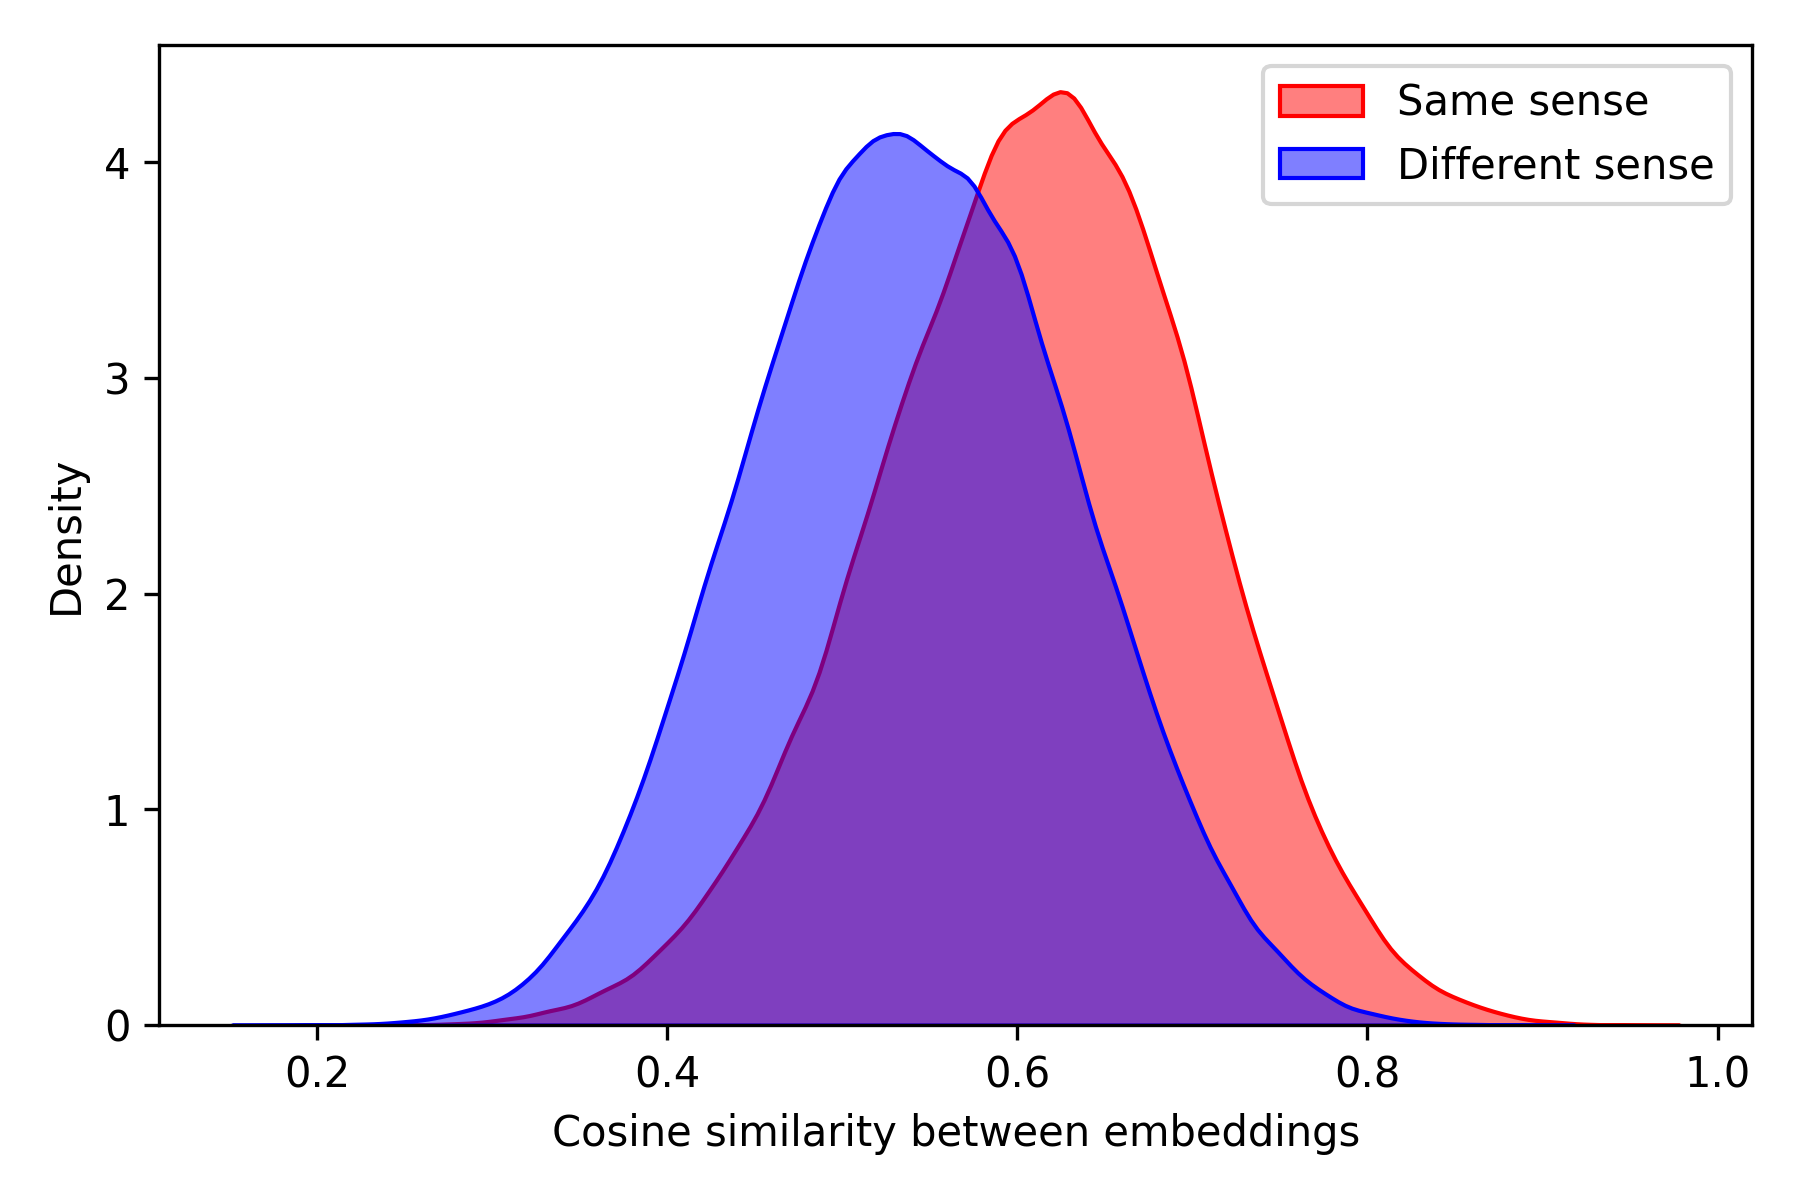
\includegraphics[width=0.5\linewidth]{../../output/plots/embedding_vs_sense_similarity_v2.png}
    \caption{Cosine similarity between same-sense and other-sense tokens of \textit{imagine}.}
    \label{fig:matrixComparison}
\end{figure}

\subsection{Senses under embedding
projection}\label{senses-under-embedding-projection}

To examine how sentence embeddings capture the annotated senses along
the three feature dimension, we trained simple linear regression models
predicting each z-scaled dimension from the sentence embeddings. The
regression coefficients define a direction in embedding space along
which the dimension increases. By projecting each sentence embedding
onto these directions, we obtain an embedding-based estimate for that
dimension. This procedure was repeated for all three dimensions,
resulting in a 3D projection of each sentence in the space spanned by
the semantic dimensions.

Here is a more detailed rundown of the analysis: Let
\(\mathbf{X} \in \mathbb{R}^{n \times d}\) denote the matrix of sentence
embeddings, where \(n\) is the number of sentences and \(d\) the
embedding dimension. Let \(\mathbf{y}^{(k)} \in \mathbb{R}^n\) be the
vector of z-scaled ratings for semantic dimension
\(k \in \{\text{intentionality, factivity, pictoriality}\}\).

We fit a simple linear regression model for each dimension:

\[
\mathbf{y}^{(k)} = \mathbf{X} \boldsymbol{\beta}^{(k)} + \boldsymbol{\epsilon}^{(k)},
\]

where \(\boldsymbol{\beta}^{(k)} \in \mathbb{R}^d\) is the vector of
regression coefficients and \(\boldsymbol{\epsilon}^{(k)}\) is the
residual vector. The estimated coefficients
\(\hat{\boldsymbol{\beta}}^{(k)}\) define a direction in embedding space
corresponding to increases in dimension \(k\).

The projection of each sentence embedding \(\mathbf{x}_i\) onto this
direction provides an embedding-based estimate of the semantic
dimension:

\[
\hat{y}^{(k)}_i = \mathbf{x}_i^\top \hat{\boldsymbol{\beta}}^{(k)}, \quad i = 1, \dots, n.
\]

By computing these projections for all three dimensions, each sentence
is represented in a 3D space spanned by the semantic directions,
allowing visualization and analysis of how embeddings capture the
annotated semantic structure.

Figure \ref{fig:3Dprojection} shows 3D projection of sentence embeddings
onto the directions corresponding to the feature dimensions. It reveals
that the sense clusters are ill-separated in this space. This indicates
that the latent embedding space does \textit{not} encode information
aligned with the feature dimensions. In other words, the directions
learned via linear regression do not effectively capture the semantic
structure underlying the sense distinctions.

\begin{figure}
    \centering
    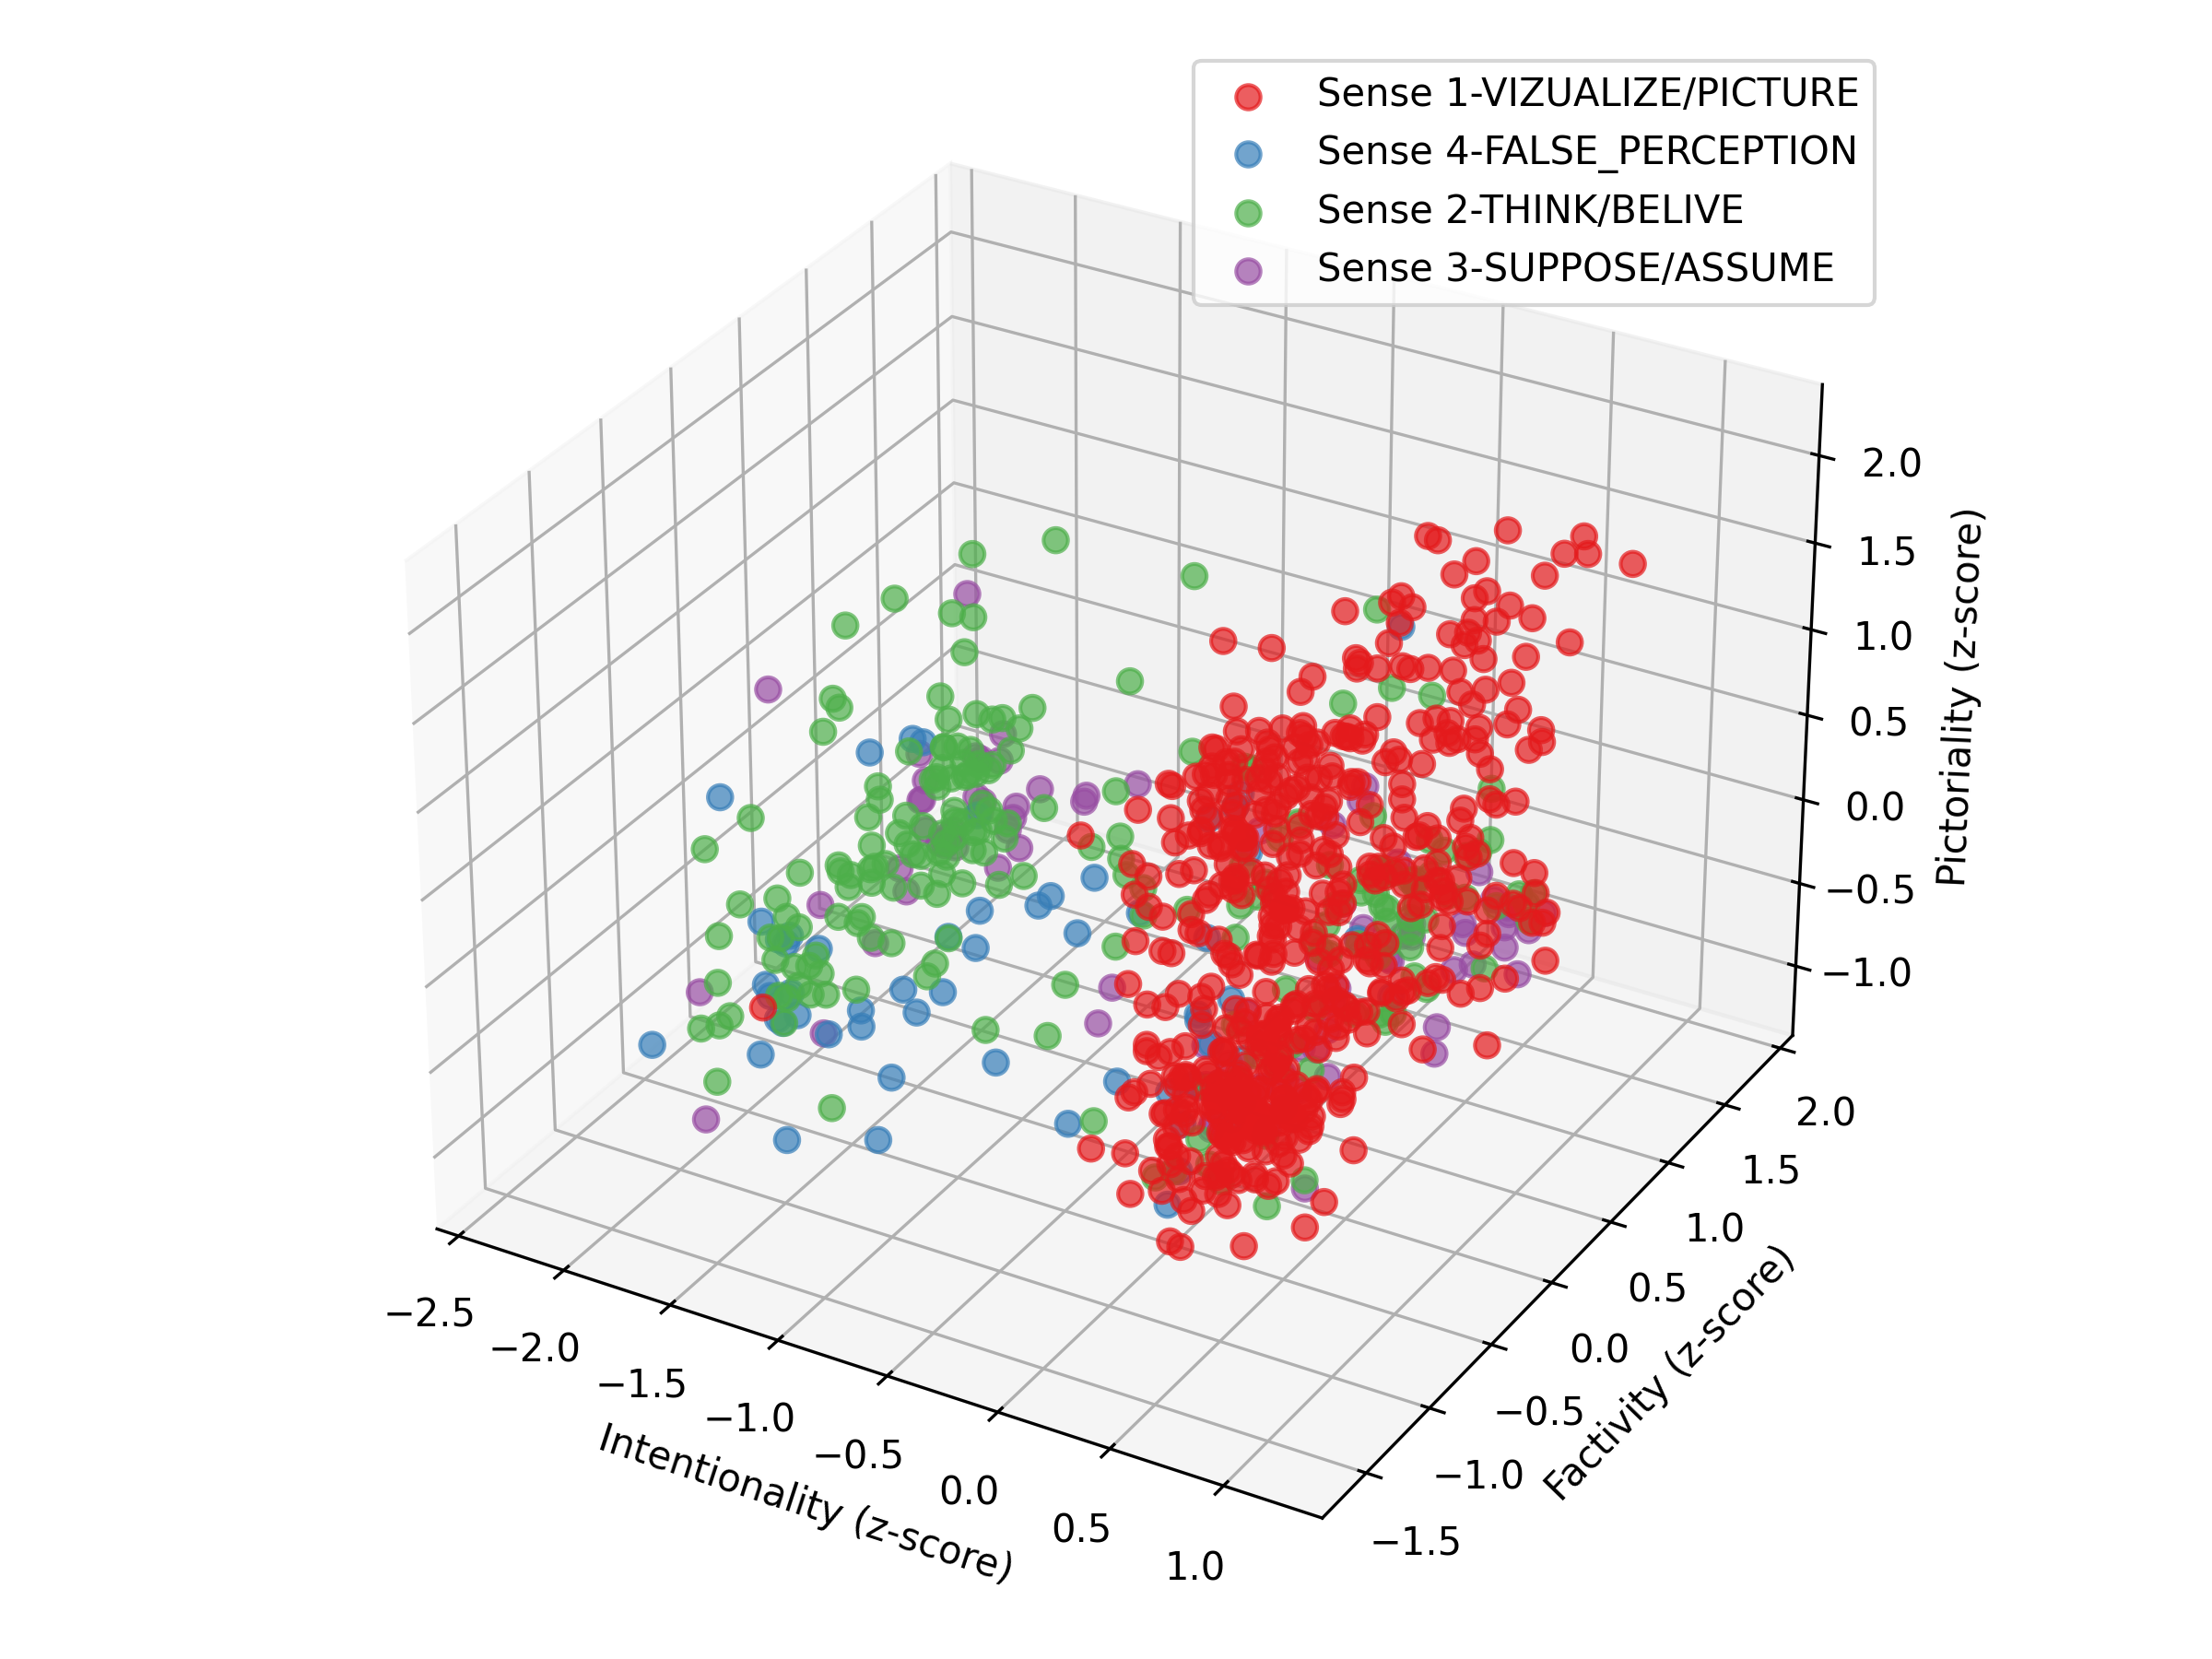
\includegraphics[width=0.5\linewidth]{../../output/plots/embedding_projection_3D_v2.png}
    \caption{3D embedding projections.}
    \label{fig:3Dprojection}
\end{figure}

Figure \ref{fig:2Dprojection} depicts 2-dimensional KDE plots for all
combinations of dimensions, supporting inseparability in 2D space.

\begin{figure}
\centering
    \caption{2D embedding projections.}
    \label{fig:2Dprojection}
    \begin{subfigure}[b]{0.30\textwidth}
    \centering
    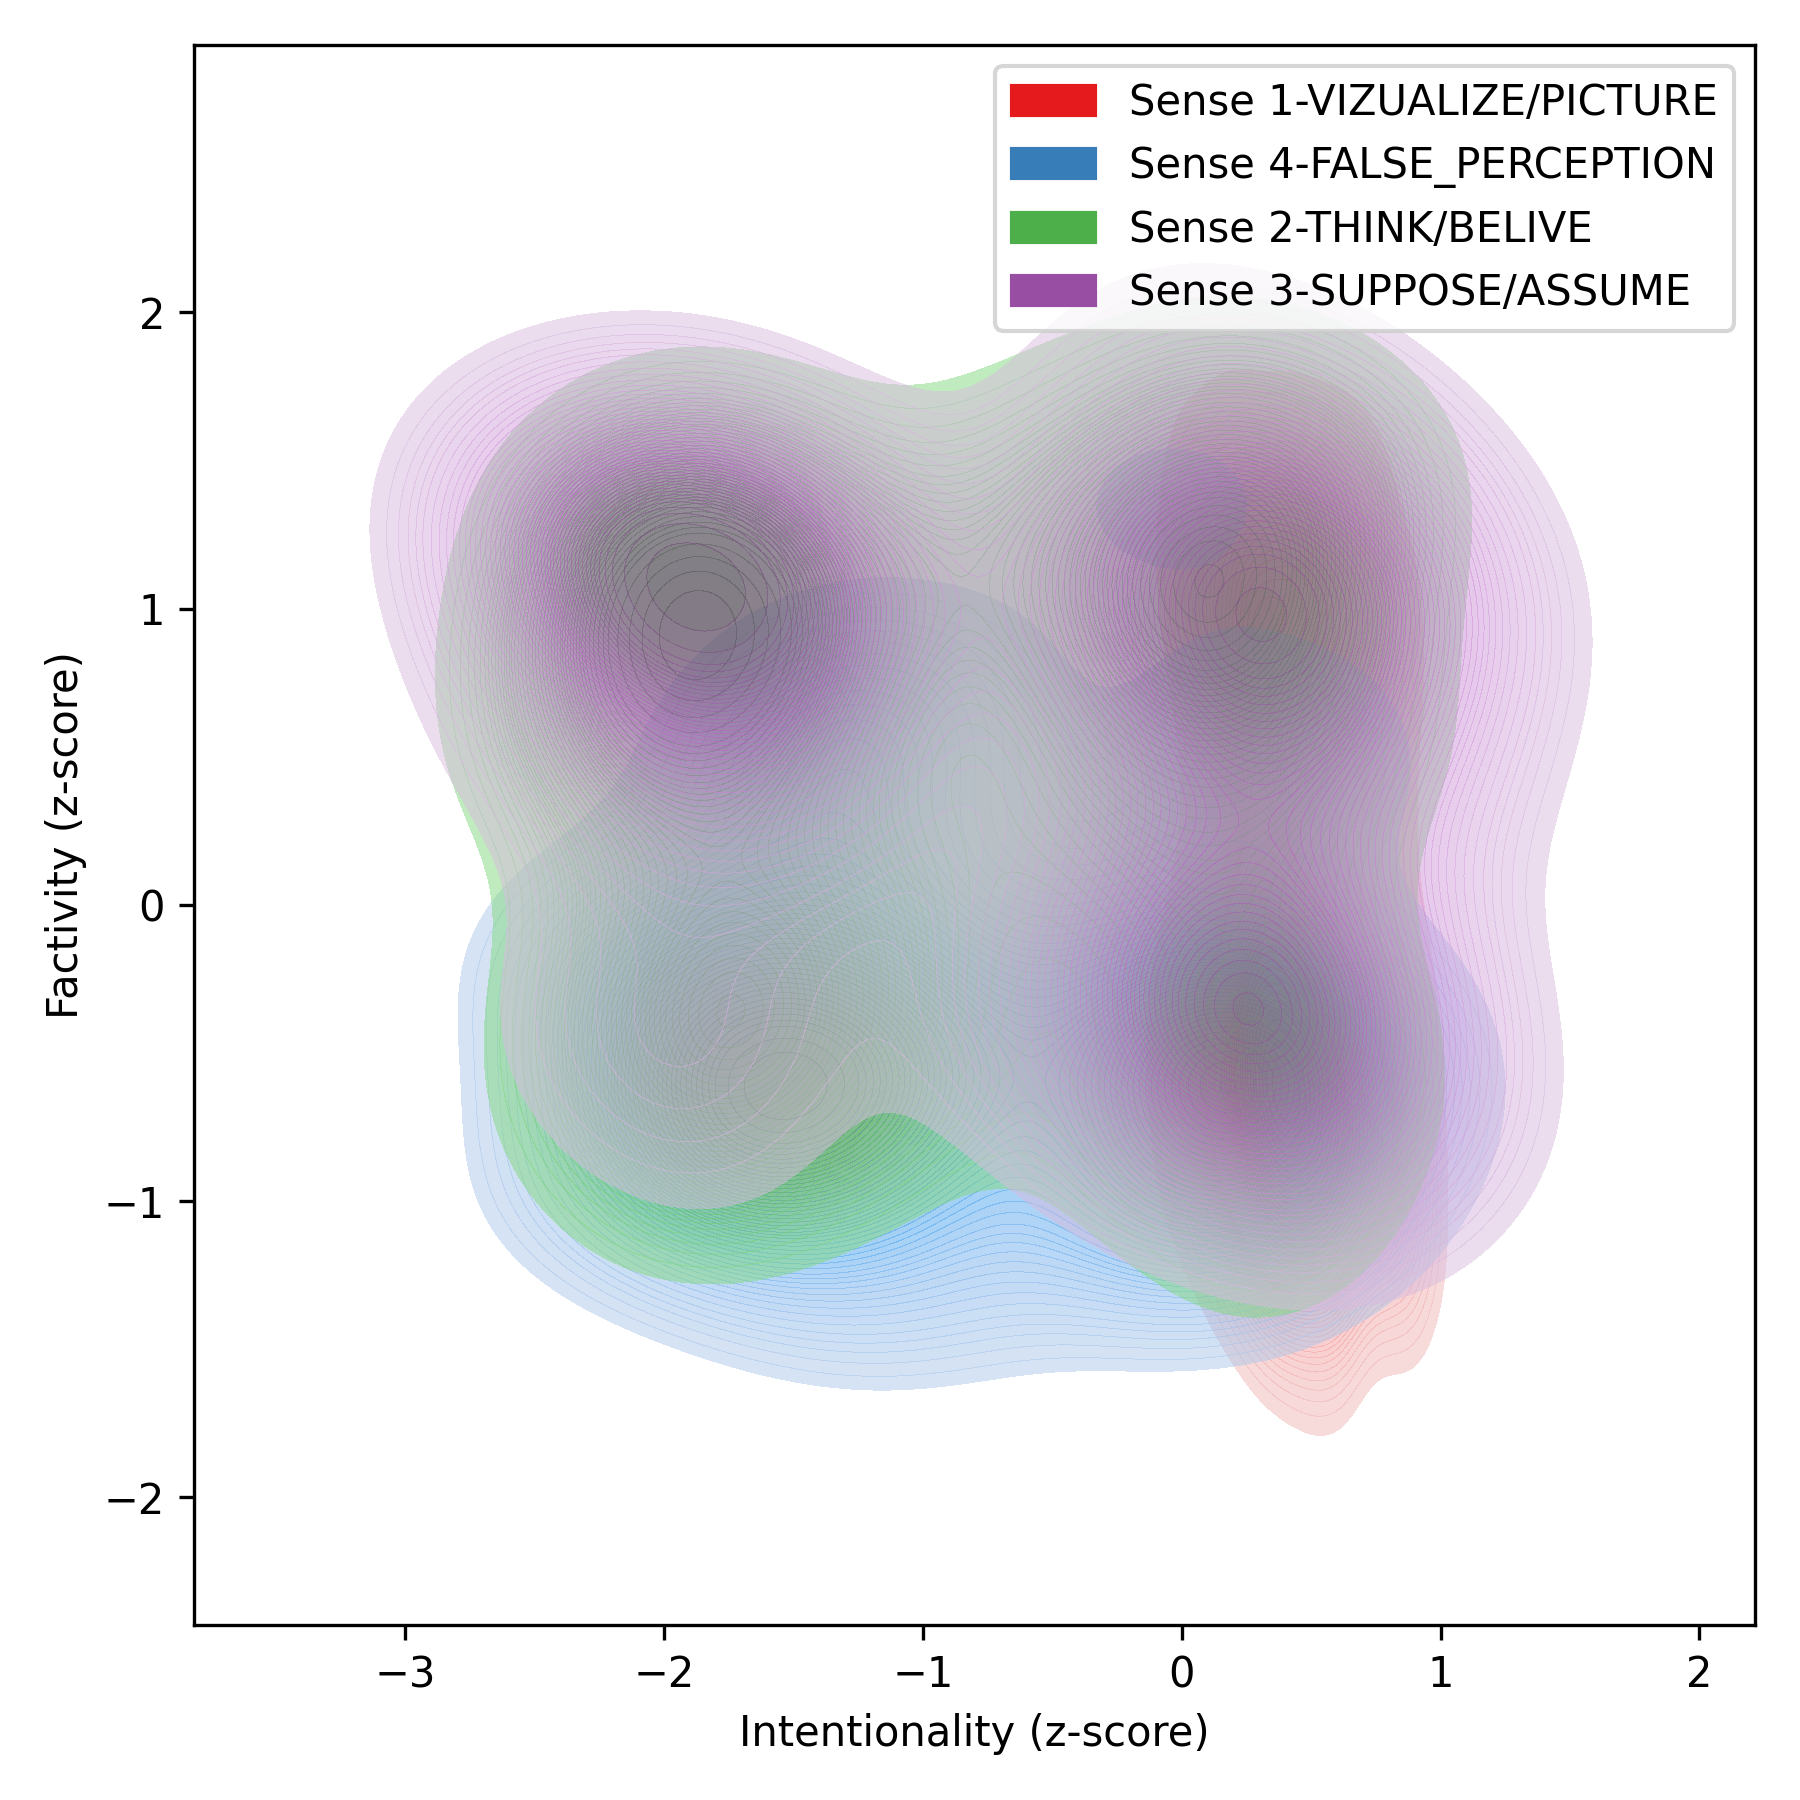
\includegraphics[width=\textwidth]{../../output/plots/embedding_projection_intentionality_factivity_2D_core_v2.png}
    \caption{Intentionality $vs$ factivity\label{fig:2D_IF}}
    \end{subfigure}
    \hfill
    \begin{subfigure}[b]{0.30\textwidth}
    \centering
    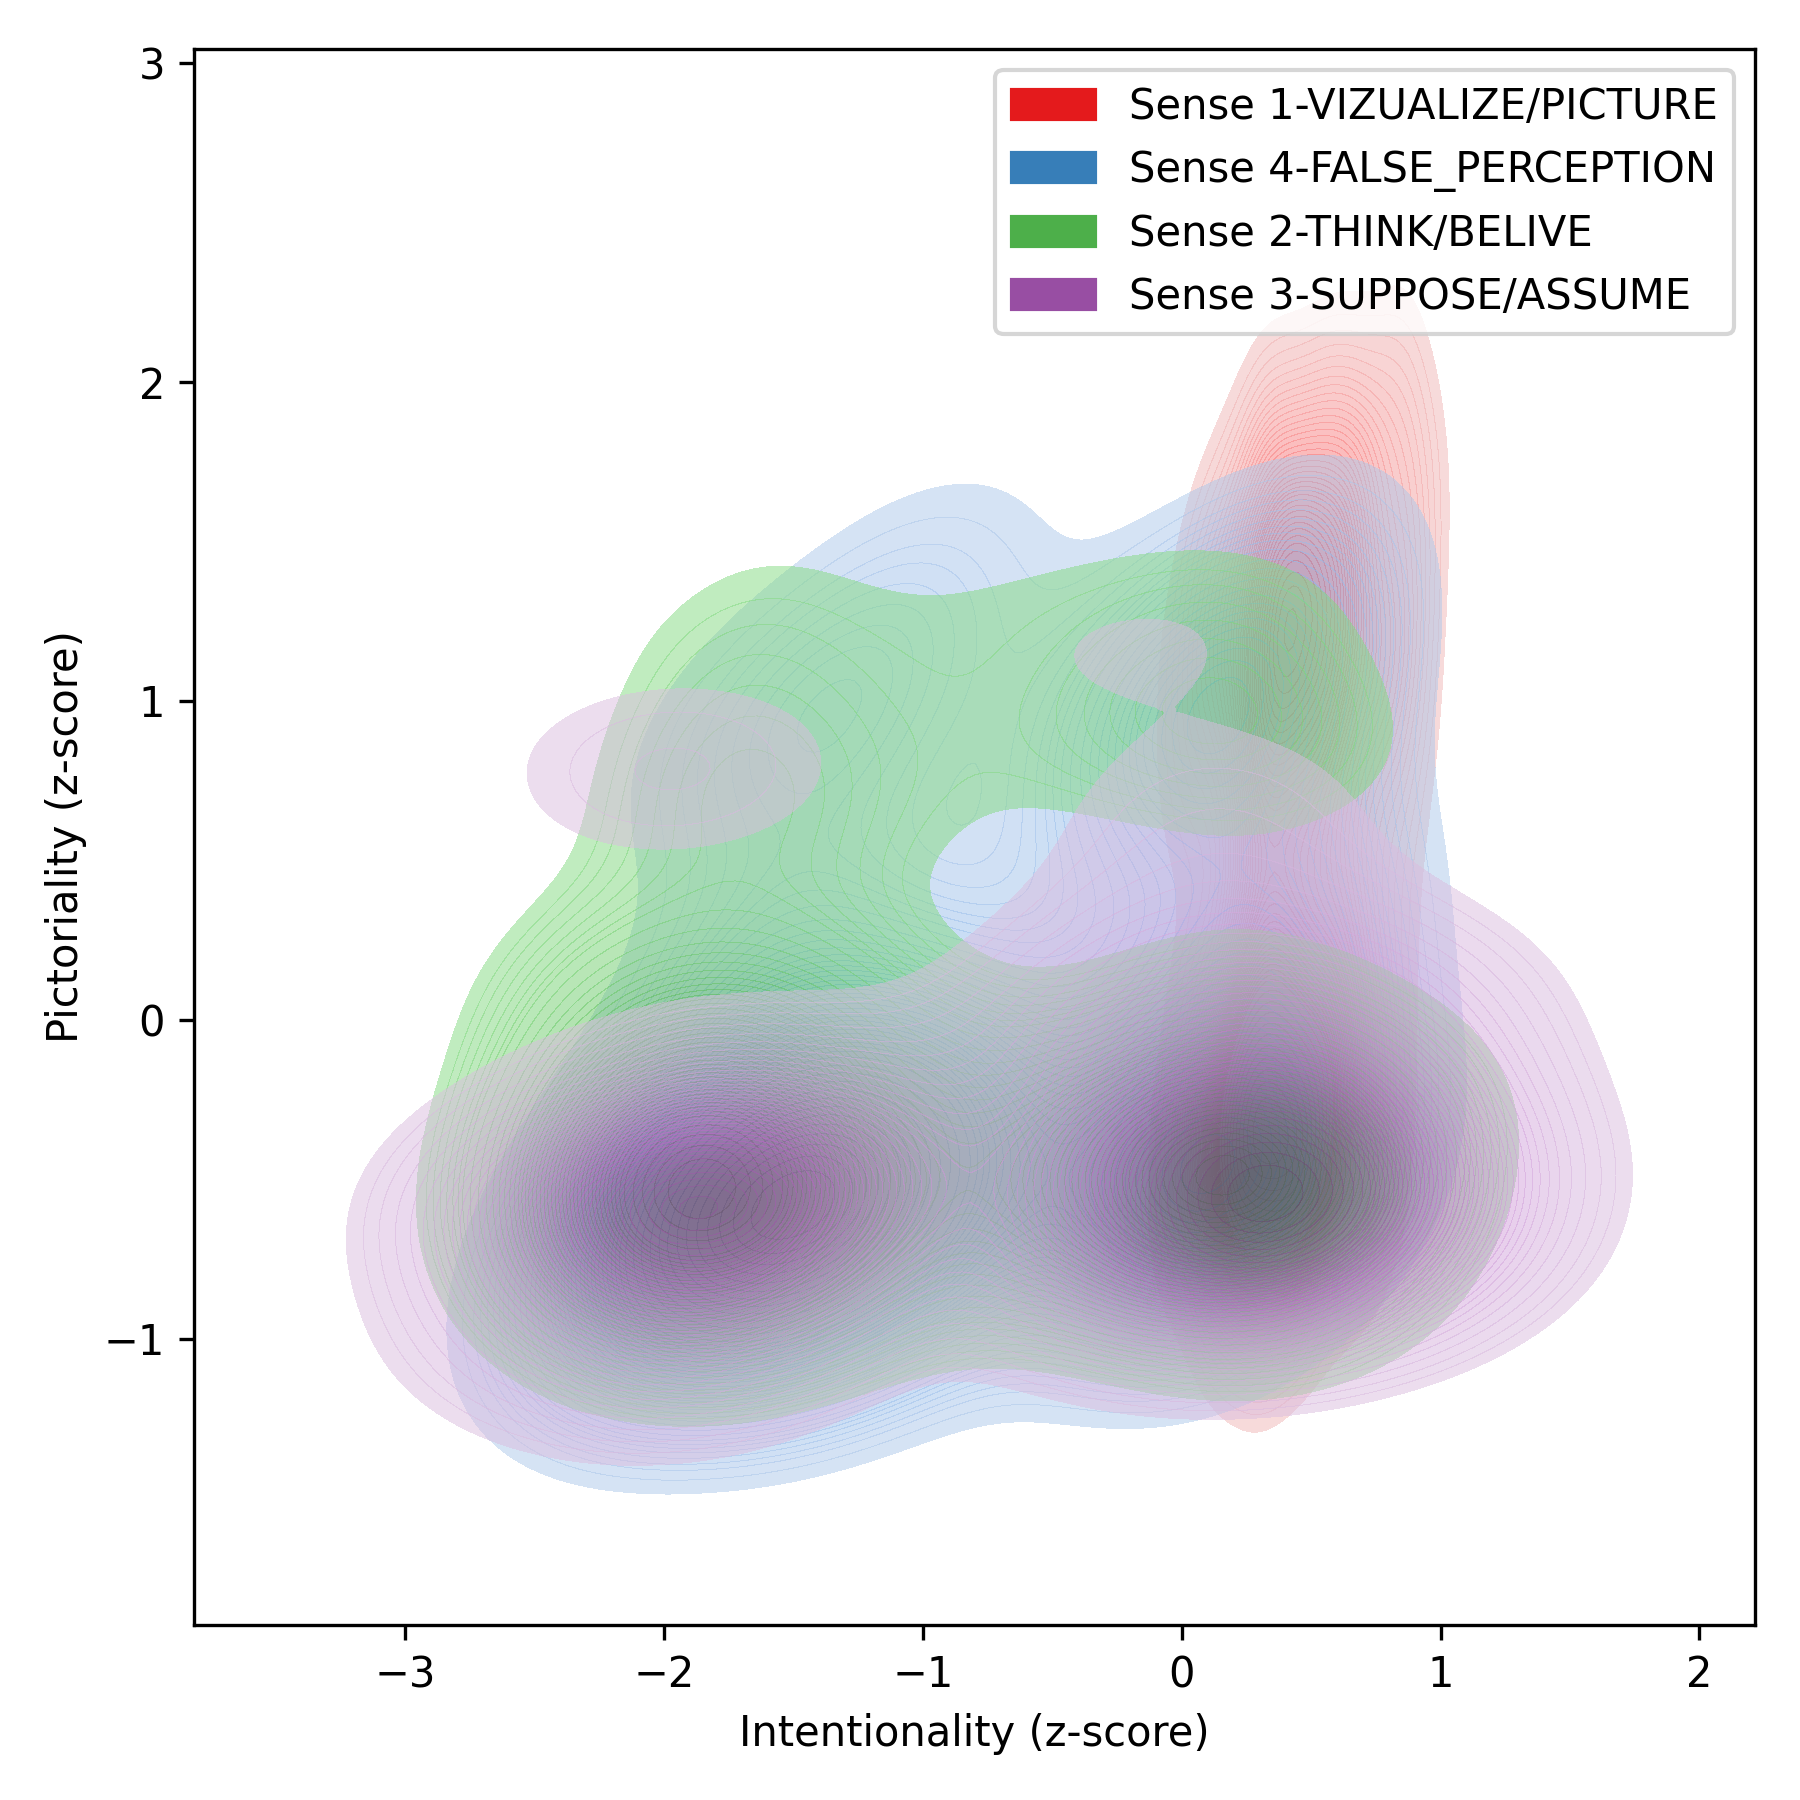
\includegraphics[width=\textwidth]{../../output/plots/embedding_projection_intentionality_pictoriality_2D_core_v2.png}
    \caption{Intentionality $vs$ pictoriality. \label{fig:2D_IP}}
    \end{subfigure}
    \hfill
    \begin{subfigure}[b]{0.30\textwidth}
    \centering
    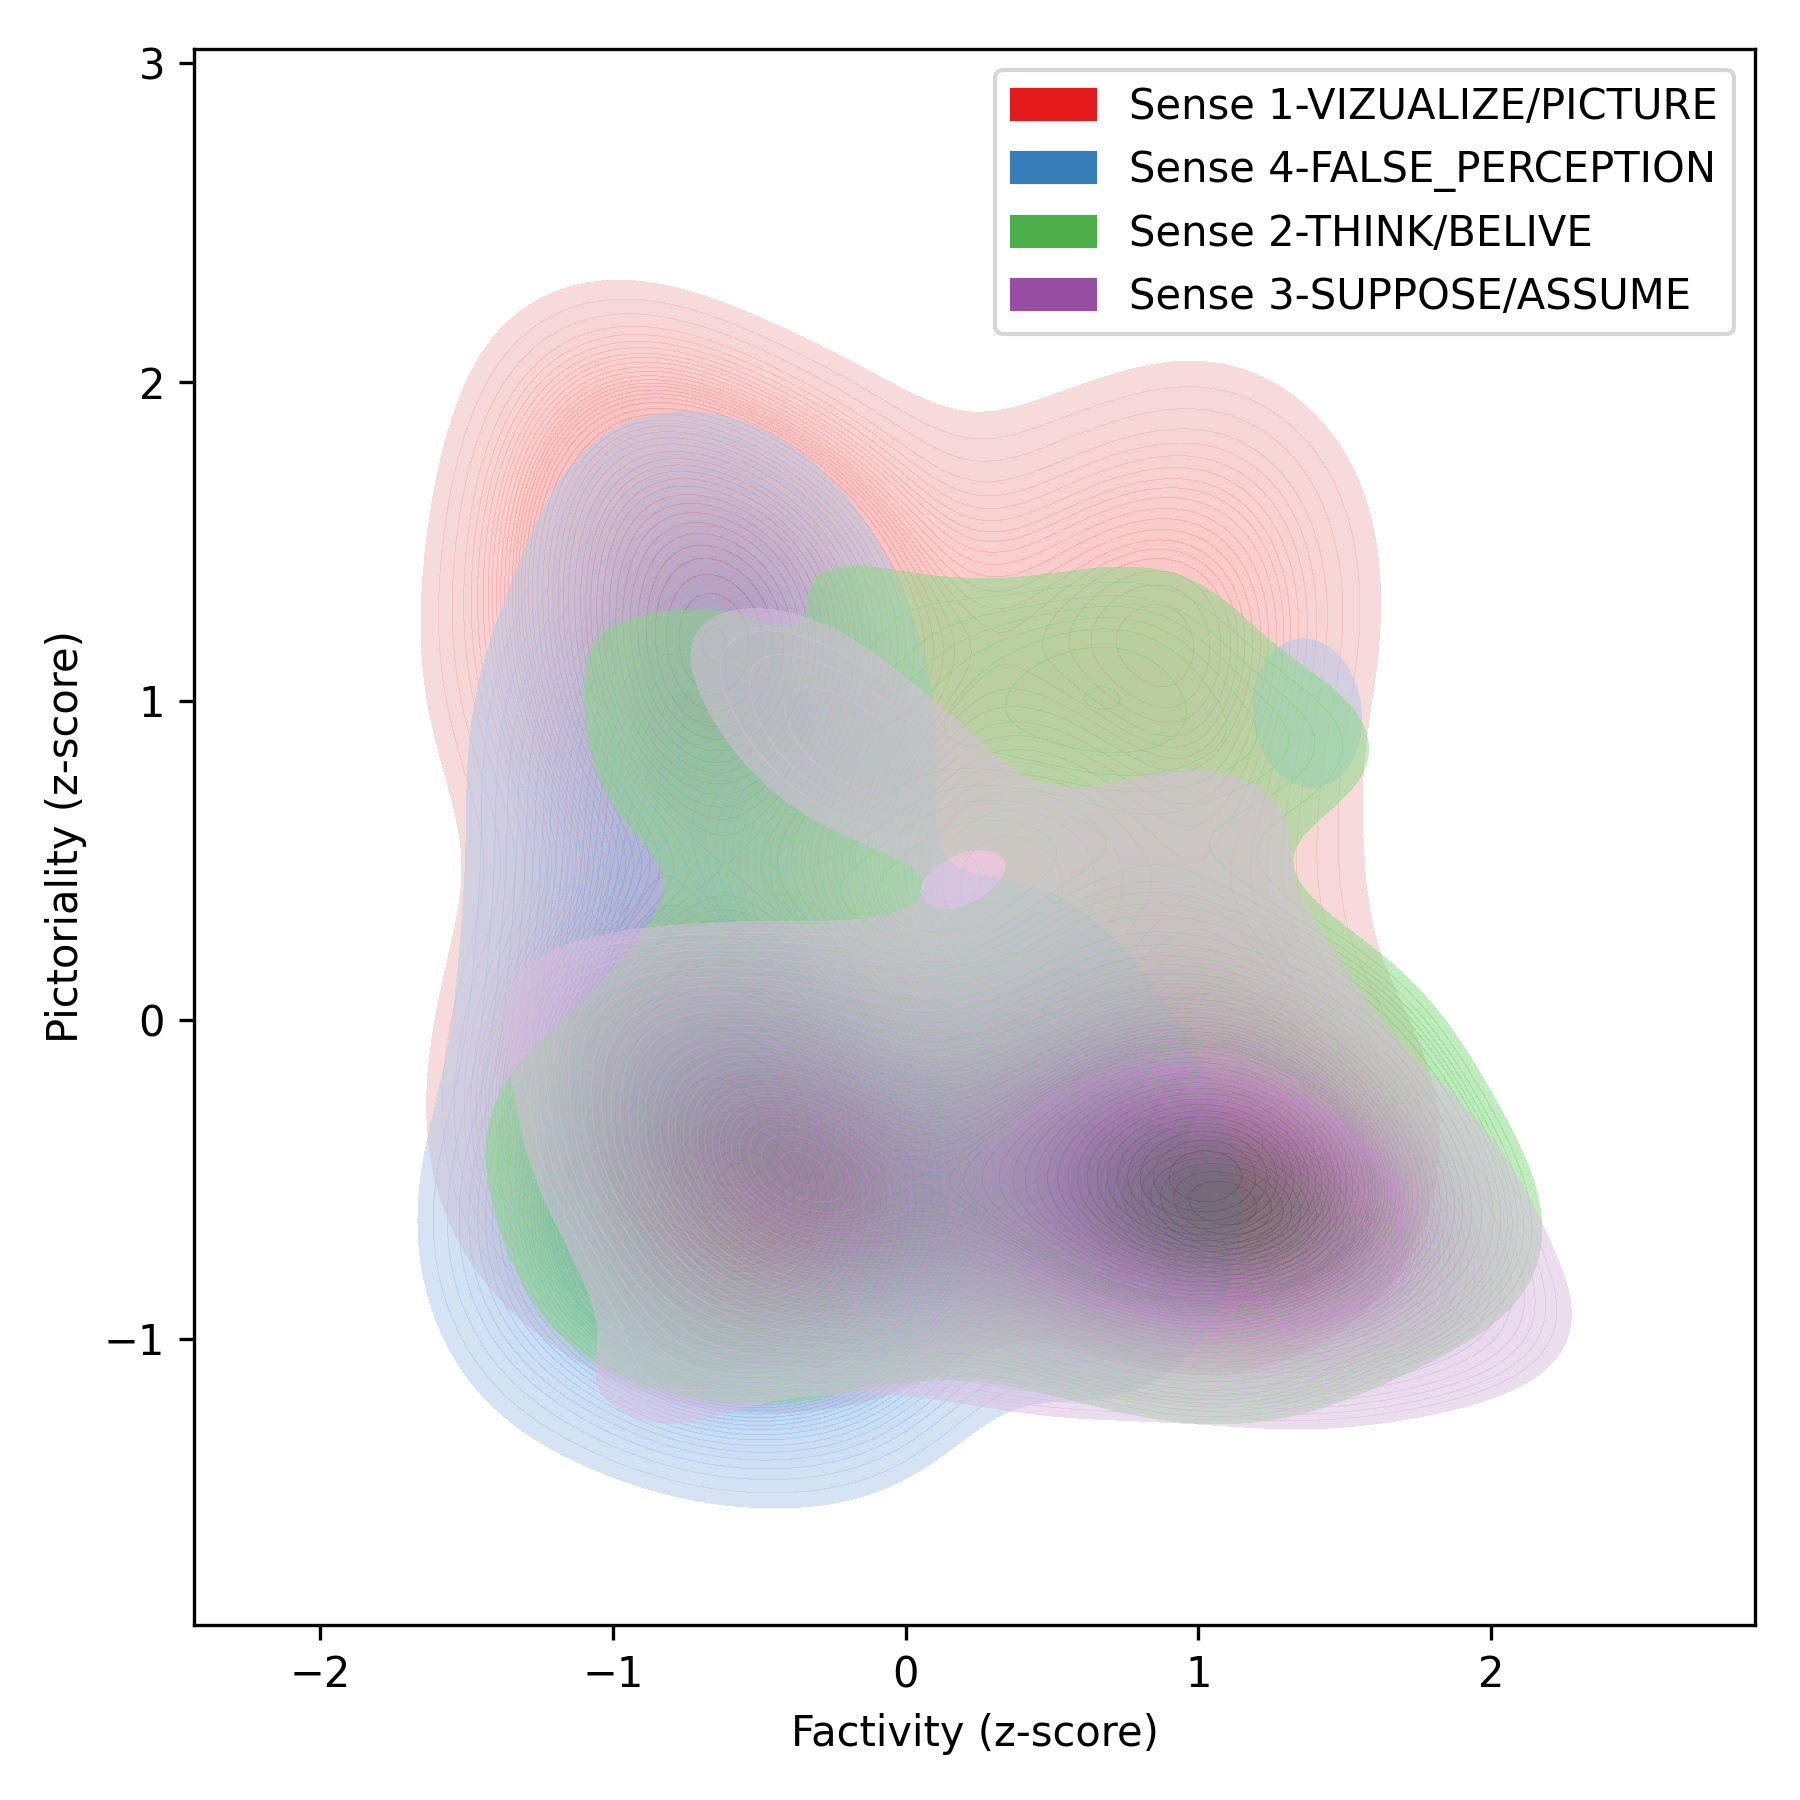
\includegraphics[width=\textwidth]{../../output/plots/embedding_projection_factivity_pictoriality_2D_core_v2.png}
    \caption{Factivity $vs$ pictoriality. \label{fig:2D_FP}}
    \end{subfigure}
\end{figure}

\section{Appendix}\label{appendix}

\begin{landscape}\begin{table}[H]
\centering
\caption{\label{tab:unnamed-chunk-14}Pairwise KDE overlap coefficients between sense distributions for each feature. 
    $\hat{O}$ denotes the raw shared area under the minimum of two KDE curves; 
    $\hat{O}_{s1}$ and $\hat{O}_{s2}$ denote the fraction of sense 1 and sense 2's 
    distribution respectively that overlaps with the other, where values approaching 1 
    indicate near-complete distributional overlap.\label{tab:overlap}}
\centering
\fontsize{8}{10}\selectfont
\begin{tabular}[t]{lllrrr}
\toprule
Feature & Sense 1 ($S_1$) & Sense 2 ($S_2$) & $\hat{O}$ & $\hat{O}_{S_1}$ & $\hat{O}_{S_2}$\\
\midrule
intentionality & 1-VIZUALIZE/PICTURE & 1-VIZUALIZE/PICTURE & 0.220 & 0.222 & 0.243\\
intentionality & 1-VIZUALIZE/PICTURE & 1-VIZUALIZE/PICTURE & 0.308 & 0.311 & 0.347\\
intentionality & 1-VIZUALIZE/PICTURE & 1-VIZUALIZE/PICTURE & 0.225 & 0.227 & 0.236\\
intentionality & 2-THINK/BELIVE & 2-THINK/BELIVE & 0.684 & 0.754 & 0.841\\
intentionality & 2-THINK/BELIVE & 2-THINK/BELIVE & 0.765 & 0.842 & 0.833\\
intentionality & 3-SUPPOSE/ASSUME & 3-SUPPOSE/ASSUME & 0.654 & 0.804 & 0.712\\
factivity & 1-VIZUALIZE/PICTURE & 1-VIZUALIZE/PICTURE & 0.597 & 0.628 & 0.625\\
factivity & 1-VIZUALIZE/PICTURE & 1-VIZUALIZE/PICTURE & 0.591 & 0.616 & 0.611\\
factivity & 1-VIZUALIZE/PICTURE & 1-VIZUALIZE/PICTURE & 0.748 & 0.786 & 0.778\\
factivity & 2-THINK/BELIVE & 2-THINK/BELIVE & 0.944 & 0.970 & 0.976\\
factivity & 2-THINK/BELIVE & 2-THINK/BELIVE & 0.406 & 0.425 & 0.422\\
factivity & 3-SUPPOSE/ASSUME & 3-SUPPOSE/ASSUME & 0.396 & 0.409 & 0.410\\
pictoriality & 1-VIZUALIZE/PICTURE & 1-VIZUALIZE/PICTURE & 0.556 & 0.597 & 0.575\\
pictoriality & 1-VIZUALIZE/PICTURE & 1-VIZUALIZE/PICTURE & 0.467 & 0.502 & 0.505\\
pictoriality & 1-VIZUALIZE/PICTURE & 1-VIZUALIZE/PICTURE & 0.665 & 0.714 & 0.737\\
pictoriality & 2-THINK/BELIVE & 2-THINK/BELIVE & 0.777 & 0.811 & 0.839\\
pictoriality & 2-THINK/BELIVE & 2-THINK/BELIVE & 0.751 & 0.784 & 0.858\\
pictoriality & 3-SUPPOSE/ASSUME & 3-SUPPOSE/ASSUME & 0.663 & 0.716 & 0.758\\
\bottomrule
\end{tabular}
\end{table}
\end{landscape}

\begin{landscape}\begin{table}[H]
\centering
\caption{\label{tab:unnamed-chunk-15}Confusion Matrix.\label{tab:cm}}
\centering
\fontsize{8}{10}\selectfont
\begin{tabular}[t]{lrrrr}
\toprule
  & 1-VIZUALIZE/PICTURE & 2-THINK/BELIVE & 3-SUPPOSE/ASSUME & 4-FALSE\_PERCEPTION\\
\midrule
1-VIZUALIZE/PICTURE & 0.9739479 & 0.2654028 & 0.5454545 & 0.3965517\\
2-THINK/BELIVE & 0.0260521 & 0.7251185 & 0.4318182 & 0.5000000\\
3-SUPPOSE/ASSUME & 0.0000000 & 0.0000000 & 0.0000000 & 0.0000000\\
4-FALSE\_PERCEPTION & 0.0000000 & 0.0094787 & 0.0227273 & 0.1034483\\
\bottomrule
\end{tabular}
\end{table}
\end{landscape}

  \bibliography{hb.bib}

\end{document}
